\documentclass[12pt, oneside]{article}   	% use "amsart" instead of "article" for AMSLaTeX format
\usepackage{geometry}                		% See geometry.pdf to learn the layout options. There are lots.
\geometry{letterpaper}                   		% ... or a4paper or a5paper or ... 
%\geometry{landscape}                		% Activate for rotated page geometry
%\usepackage[parfill]{parskip}    		% Activate to begin paragraphs with an empty line rather than an indent
\usepackage{graphicx}
\usepackage{xcolor}				% Use pdf, png, jpg, or eps§ with pdflatex; use eps in DVI mode
								% TeX will automatically convert eps --> pdf in pdflatex	
\usepackage{amssymb, amsmath,amsthm}

\newtheorem{thm}{Theorem}
\newtheorem{defn}{Definition}
\newtheorem{claim}{Claim}
\newtheorem{assumption}{Assumption}

\graphicspath{{figures/}}	

\author{Michael J. Collins\\Senior Analyst, Daniel H. Wagner Associates\\mjcollins10@gmail.com}
\title{Calculus, A Little Bit Differently}
\date{}
\begin{document}

%consider defining in terms of open intervals rather than delta (but mention that \pm\varepsilon is easiest way to define an 
%interval and use this in proofs. Either way switch to notation that makes dependence of N on \varepsilon obvious,
%either $N_{\varepsilon}$ or $N_I$ where $I$ is an open interval.

%%TODO: all fig/thm numbers should be derived from section/subsection numbering

%what to do with this? Springer author site says "We typically publish textbooks at the advanced undergraduate and graduate level so we are not looking for core first-year undergraduate textbooks". That rules out calculus, although they do publish introductory combinatorics. Look into other options; or just put it online and try to get some buzz going from Rich's email list and branch out from there. Wiki textbooks? They have calc already of course -- room for two? Or just a link to my stuff -- must be on github (with large-file plugin for PDF diagrams).
%Should we try to get some physics applications and programming exercises in there?
%If we have publicly available link, must make sure we link to clean version with reasonably complete sections

%leanpub.com looks promising; closely linked to openIntro which already has "apex calculus" by Gregory Hartman;
%that book features interactive graphics (definitely something a modern calc text should have), and uses the hyperref
%package so every mention of theorem a.b links to that theorem etc. Feel out of my depth in trying to create decent
%graphics -- but the whole thing is on github, so can try just stealing some of their stuff! and Hartman can be reached at
%apexcalculus@gmail.com

%There is now a fourth edition of Spivak (July 2008), should compare although I doubt the underlying structure has changed. Should look at more application-oriented books to see what sort of examples they use and how they handle/evade the theoretical issues. Also Amir Babak Aazami's "48 Hours of Honors Calculus" is another attempt at something at Spivak's level; he also begins with the limit of a sequence, but zips through the foundations more quickly and even defines continuity in terms of open sets! (and the actual definition of derivative is the standard one). So I cannot claim that starting with sequences is novel; Amazon preview does not show how he gets from sequences to $\lim_{x \to a} f(x)$, but it is clear from exercise 4.14 (pg. 80). that he does use the classic epsilon/delta definition of $\lim$. Would be worth $40 to buy this one.

\maketitle
Dedicated to my high-school math teacher Robert Sikso, who said ``no, stick with this, I think you can do it" when I wanted to drop my freshman advanced algebra class because I was finding it difficult.


\section*{Introduction for Instructors and Mentors}
This text covers the standard material of a differential calculus course, but it departs from convention by taking the \emph{limit of a sequence at infinity} as the most fundamental concept; derivatives and continuity are defined in terms of such sequences, while the notion of ``the limit of $f(x)$ as $x \to a$'' does not appear. The treatment of limits emphasizes the notion of open intervals.

Trigonometric functions and their derivatives are treated in a  geometric (but rigorous) manner.
The more subtle properties of the real numbers (i.e. the Archimedean property and convergence of Cauchy sequences) are introduced as needed, in contexts where they arise naturally. %I have generally avoided proofs by contradiction. 

 I hope that many students will find this approach helpful.  I think that ``$\lim_{x \to a}f(x)$" is rather artificial in elementary calculus, since for all ``normal'' functions  this is just $f(a)$; in the first two chapters I believe I present a convincing case for taking sequences and series as the starting point. %The extensive use of open intervals might be seen as an introduction to topology, but that was not my motivation; the notion of ``an interval with the endpoints missing'' is no more abstract than anything else students have to absorb here, and the use of intervals simplifies many proofs.
%in fact, so far have not had as much emphasis on open intervals as I had anticipated
There are other texts which put sequences and series first (\emph{48 Hours of Honors Calculus} by Amir Babak Aazami) but I do not know of any that define derivatives and continuity in terms of sequences and bypass $\lim_{x \to a}f(x)$.
%I do not know of any other textbook which puts topics in this order, although this way of looking at things has much in common with the approach based on infinitessimals -- while avoiding the technical difficulty of figuring out what an infinitessimal number is. 

I acknowledge a great debt to Michael Spivak's \emph{Calculus}, a model of clear exposition and the source from which I learned the subject.

{\color{red}Descriptions of sections that still need to be written are printed in red, although at this point almost every section needs more exercises and additional figures.}


\section*{Preface}
This book covers the standard material for a course in differential calculus, taking a somewhat different approach from other textbooks. If you compare it to a standard text, you will see that the definitions I give for basic concepts -- ``continuous function", ``derivative" et cetera -- look different. But all these definitions \emph{mean} exactly the same things -- a function is ``continuous" by this book's definition if and only if it is continuous according to the standard definition et cetera. I have restated the classic definitions in a way that I hope is easier to understand, simpler, and more focused on fundamental concepts. But I have not just changed the wording of definitions; the new definitions require us to cover topics in a rather different order from other books, and lead to different choices about what topics to emphasize. 
 
Calculus inherently requires a solid understanding of algebra. Students studying calculus are typically familiar with standard high-school problems such as solving for $x$ in a quadratic equation like
\[
x^2 - 3x + 2 = 0 
\]
or solving for $x,y$ in a system of  linear equations like
\begin{align*}
2x +& 5y = 0\\
-x -& 8y = 3
\end{align*}
et cetera. More generally, the reader will have to be comfortable with manipulating algebraic expressions and inequalities. %I have not included and refresher material on pre-calculus, since such review is available elsewhere.%If you work through all the exercises, you should end up being quite adept at such manipulations! 

%This text gives only passing mention to applications of calculus in science and engineering. To really give convincing applications of mathematical theory in some particular domain requires a fairly deep exploration of  that domain, which is not possible here.  So I just ask the reader to take it for granted that when we sometimes motivate our equations by saying that they describe the motion of an object, or some other quantity varying in time or space, we are talking about things of fundamental importance in the physical sciences.

\pagebreak
\section{Limits}
\subsection{A First Example}
Our point of departure is the familiar equality 
\[\label{eq:onethird}
\frac{1}{3} = 0.333\cdots\ 
\]
where the dots mean that the decimal goes on forever repeating the digit ``3". We take this for granted, but really there is something odd here; infinity is a rather profound concept, so why do we need an infinitely long number -- something nobody could ever even write down! -- to express something as straightforward as dividing one by three? The answer is that we have no choice: any finite sequence of 3s is too small, but as soon as we write a 4 it is too large. There is no finite decimal which comes out to \emph{exactly} one-third. 

When using numbers to measure things, this is not a problem, because physical measurements are never exact. How many decimal places we care about depends entirely upon what we are doing. For a carpenter cutting a board, there is no meaningful difference between 0.33 inches and a third of an inch; if we are guiding a spacecraft there is no real difference between $\frac{1}{3}$ kilometer and 0.3333333 kilometers, as these differ by less than the width of a hair. So in general we do not need many decimal places to get \emph{very} close. There is no way to put a strict bound on the largest number of decimal places we might ever need, but no matter how much accuracy we seek, we can always get there. 

This notion of a sequence of ever-better approximations, which can eventually attain any required level of accuracy, is in fact the essential idea which will be the basis for everything we do in calculus. Before diving into general definitions, we will restate more precisely what we mean by  ``approximation". When we assert that $0.333\cdots = \frac{1}{3}$, what we are really claiming is this:

\begin{thm}\label{thm:onethird}
Let $\varepsilon$ be any number greater than 0. There exists some integer $N$ such that
\[
\frac{1}{3} - 0.\underbrace{33\cdots3}_\text{$N$ times} < \varepsilon 
\]
\end{thm}

The idea here is that $\varepsilon$ is the required ``degree of accuracy", or ``error tolerance" for our approximation. We must exclude $\varepsilon=0$ because that would mean perfect accuracy -- which is not possible. But anything short of perfection is possible -- which is why we can say \emph{any} $\varepsilon>0$. 

We prove our claim in the straightforward way -- by explicitly calculating the required number of digits $N$ (which depends on $\varepsilon$). Smaller $\varepsilon$ means more accurate approximation, which requires larger $N$. To start we can get rid of fractions (often a good thing to do when manipulating algebraic expressions) by multiplying both sides of the inequality by 3; now we have to find $N$ such that
\[
1 - 0.\underbrace{99\ldots9}_\text{$N$ times}  < 3\varepsilon 
\]
i.e
\[
10^{-N} < 3\varepsilon 
\]
And of course we can always find such an $N$; if the decimal expansion of $3\varepsilon$ starts with, say, 47 zeros, take $N>47$ and so on. 

The important thing about this proof is that the vague notation ``$\cdots$" is gone; we have stated everything in terms of inequalities involving finite expressions. The only point at which infinity enters the picture is in considering \emph{all} of the infinitely many finite expressions we could imagine writing.  This typifies the kind of reasoning we will use to deal with infinity. 

We should note that the ``infinity" of $0.33\ldots$ is avoidable and somewhat artificial, since we already have a perfectly good finite way of writing down this quantity, i.e. ``$1/3$". \footnote{And if we used base-3 instead of base-10, we would write this number finitely as ``0.1".}
Reasoning about infinity will become truly essential when we consider numbers that inherently cannot be represented as fractions,  like $\sqrt{2}=1.4142135623730951\cdots$ or  $\pi = 3.1415926\cdots$.\footnote{If the fact that these numbers cannot be fractions is unfamiliar to you, see section \ref{sec:sqrtIrrational}}

\subsection{Exercises}
\begin{enumerate}
\item In the same manner as Theorem \ref{thm:onethird}, prove that
	\begin{itemize}
	\item $1/9 = 0.11111\ldots$
	\item $1/7=0.142857142857142857\ldots$
	\end{itemize}
\item Considering the previous exercise, how might you figure out the decimal expansion of $1/11$ without a calculator?
\item Express .027027027... as a fraction. 
\end{enumerate}


\subsection{Definition of Limits}
So far we have considered approximations stated in terms of ever-longer decimal expansions, but that is just because decimals are  familiar and easy to deal with. In fact there is nothing special, or even particularly important, about decimal expansions. Certainly the sequence $3.1, 3.14, 3.141, \ldots$ keeps getting closer to $\pi$, but there are many other ways to get there. One well-known approximation starts with $\frac{22}{7}$, followed by $\frac{333}{106}$, then $\frac{355}{113}$; we are not ready yet to explain where these numbers come from, but you can do the division and see that these fractions are close to the familiar $3.1415926\cdots$.

We have been speaking informally about ``sequences" of numbers, but since these will be so important we need a definition. A sequence is an infinite ordered list of real numbers, usually written with subscripts to show where in the list we are: $a_0,a_1, a_2, a_3 \cdots$ et cetera (whether we start at one or zero does not much matter, but more often we start at zero). More formally, a sequence is a function mapping the natural numbers to the real numbers.

We now state our most fundamental definition, which generalizes the concept behind theorem (\ref{thm:onethird}):
\begin{defn}\label{def:limit}
Let $a_0,a_1,a_2,\ldots$ be a sequence of real numbers. The real number $A$ is the \emph{limit} of this sequence if,
for each $\varepsilon > 0$, there exists an integer $N_\varepsilon$ such that
\[
|A - a_n| < \varepsilon 
\]
whenever $n \geq N_\varepsilon$. We write this as
\[
\lim a_n = A
\]
\end{defn}
We use absolute value because it does not matter whether $a_n$ is smaller or larger than $A$, all that matters is that they are in some sense \emph{close}; the absolute value gives us the \emph{distance} between two numbers, which is what we need. 

%I do not think we have actually used this language anywhere -- will we?
%Whenever there is an $N$ such that some proposition $P(n)$ holds whenever $n>N$, we may say that ``$P(n)$ is eventually true" or, more tersely, ``eventually $P(n)$". The use of the word ``eventually" suggests the passage of time; in general there is no reason why larger $n$ in $a_n$ has to refer to  later moments in time, but it is often natural to think of things this way, as if the terms of a sequence are being revealed in order.

A sequence which has a limit is said to \emph{converge}, or to be convergent; a sequence which does not converge is \emph{divergent}. So theorem (\ref{thm:onethird}) can be restated as asserting that the sequence
\[
a_n = \frac{3}{10} + \frac{3}{100} + \cdots + \frac{3}{10^n}
\]
converges to $1/3$, i.e. that $\lim a_n = 1/3$.
Note that $a_n$ is defined as the sum of the first $n$ terms of yet another sequence (i.e. $b_k=\frac{3}{10^k}$); we will see in the next chapter that many other sequences are defined in this way.

We will see many examples of sequences which do and do not converge, and will use convergence as the basis for other definitions. But first we give another example of how to find the limit of a sequence.

\begin{thm}\label{thm:oneOverN}
Let $a_n = \frac{1}{n}$. Then
$\lim a_n = 0$.
\end{thm}
We usually simplify the notation and just write this as $\lim \frac{1}{n} = 0$.
We must prove that, for any $\varepsilon > 0$, we have 
\[
|0 - 1/n| < \varepsilon
\]
when $n$ is larger than some yet-to-be-determined $N_\varepsilon$. This can be written more simply as
\[
1/n < \varepsilon
\]
and so 
\[
n > 1/\varepsilon
\]
Thus we take  $N_\varepsilon$ to be (at least) the next integer past $1/\varepsilon$ (which will be large when $\varepsilon$ is small).

Not every sequence of numbers has a limit; a sequence like $a_n=(-1)^n$ (i.e. 1,-1,1,-1,1,$-1\cdots$) that bounces around rather than settling down close to one particular value is a good example.
To prove this, we must show that no real number could satisfy our definition.
For instance we cannot have $\lim a_n =1$; taking $\varepsilon = 1/2$, no matter how large $N$ is there will always be $n>N$ for which $a_n = -1$ so $|a_n - 1| > 1/2$.
All other numbers can be dismissed similarly.%\footnote{With this you have reached a true epoch in your mathematical education; problems for which it is not always easy to figure out if there even is an answer. You might want to mark this occasion with appropriate ceremony. But please no underage drinking.}

A sequence can also fail to have a limit by going off to infinity, for instance $a_n=n$. No real number $X$ could be the limit; for any $\varepsilon$ we will have $a_n>X+\varepsilon$ if $n>X+\varepsilon$.

\subsection{Exercises}
\begin{enumerate}
\item Finish the proof that  $(-1)^n$ does not have a limit
\item Prove that $\lim 17/n^2 = 0$
\item Evaluate $\lim \frac{n-42}{2n-1}$
\item Restate the results from the first set of exercises in terms of limits.
\end{enumerate}


The proof of theorem \ref{thm:oneOverN} actually merits a bit more scrutiny.
We have taken it for granted that, for every real number (the real number $1/\varepsilon$ in this case), there exists a larger \emph{integer}; this is called the ``Archimedean property" of the real number system.
This seems rather obvious and is indeed true; it is another way of saying there are no ``infinitely large" numbers that cannot be reached with a finite number of fixed-size steps\footnote{It also means there are no ``infinitessimally small" numbers that cannot be added up to reach something large.}. 
But it is an assumption and should be explicitly identified as such, along with more familiar assumptions like the commutative and distributive properties. We will see other results that require the Archimedean property later in the chapter.

\subsection{Exercises}
\begin{enumerate}
\item The proof that $a_n=n$ diverges also implicitly used the Archimedean property; where?
\item Prove that $\lim 17/n^2 = 0$
\item Evaluate $\lim \frac{n-42}{2n-1}$%need to show example of n/(n+1)
%\item $\lim nx^n = 0$ for any $x$ such that  $|x|<1$.
\item $\lim \frac{n^2}{2^n} = 0$
\end{enumerate}


\subsection{Basic Properties of Limits}
To work with limits we will need to establish some of their  basic properties. We will put the possibility of non-convergence aside for the moment, and focus on what must be true about limits when they do exist. The most fundamental property of limits is that they are \emph{unique}: given $a_n$, if there is \emph{any} number $A$ satisfying definition (\ref{def:limit}), then there is only one such number. This is why we always speak of \emph{the} limit of a sequence. 

\begin{thm}\label{thm:uniqueness}
Suppose that $A$ is a limit of $a_n$ -- i.e. that $A$ and $a_n$ satisfy definition (\ref{def:limit}). Then no other number is a limit  of $a_n$.\end{thm}

\begin{proof}
Let $B\neq A$; we must show that $B$ is \emph{not} a limit of $a_n$. The idea is to make $\varepsilon$ smaller than the gap between $A$ and $B$. By definition, once $n$ gets large enough the sequence will then stay in the open  interval\footnote{If you have not encountered this term before, the \emph{open} interval $(a,b)$ is the set of all numbers between $a$ and $b$, \emph{excluding} the endpoints $a,b$. If we include the endpoints we have a \emph{closed } interval, written $[a,b]$} $(A-\varepsilon,A+\varepsilon)$; that is just another way of saying $|a_n-A|<\varepsilon$. Since $B$ is outside this interval, the sequence will not stay ``close" to $B$ when $n$ is this large. Now let us work through this idea more carefully. 

Choose $\varepsilon, \varepsilon'$ so that the intervals $(A-\varepsilon,A+\varepsilon)$,   $(B-\varepsilon',B+\varepsilon')$ do not overlap. It is clearly possible to do this; looking at diagram (\ref{fig:uniqueness}), we can see that what we require is $\varepsilon+\varepsilon' \leq |A-B|$.  Let $N$ be a number (known to exist by assumption) such that $n>N$ implies $|a_n-A|<\varepsilon$.  Now could there be an $N'$ such that $n>N'$ implies $|a_n-B|<\varepsilon'$? No! Whatever $N'$ is, we could have $n$ greater than \emph{both} $N'$ and $N$ -- i.e. $n>\max(N,N')$. Then we must have  $a_n \in (A-\varepsilon,A+\varepsilon)$, in which case $a_n \not\in (B-\varepsilon',B+\varepsilon')$. The non-existence the required $N'$ means that $B$ is not a limit of $a_n$.
\end{proof}

\begin{figure}
\begin{center}
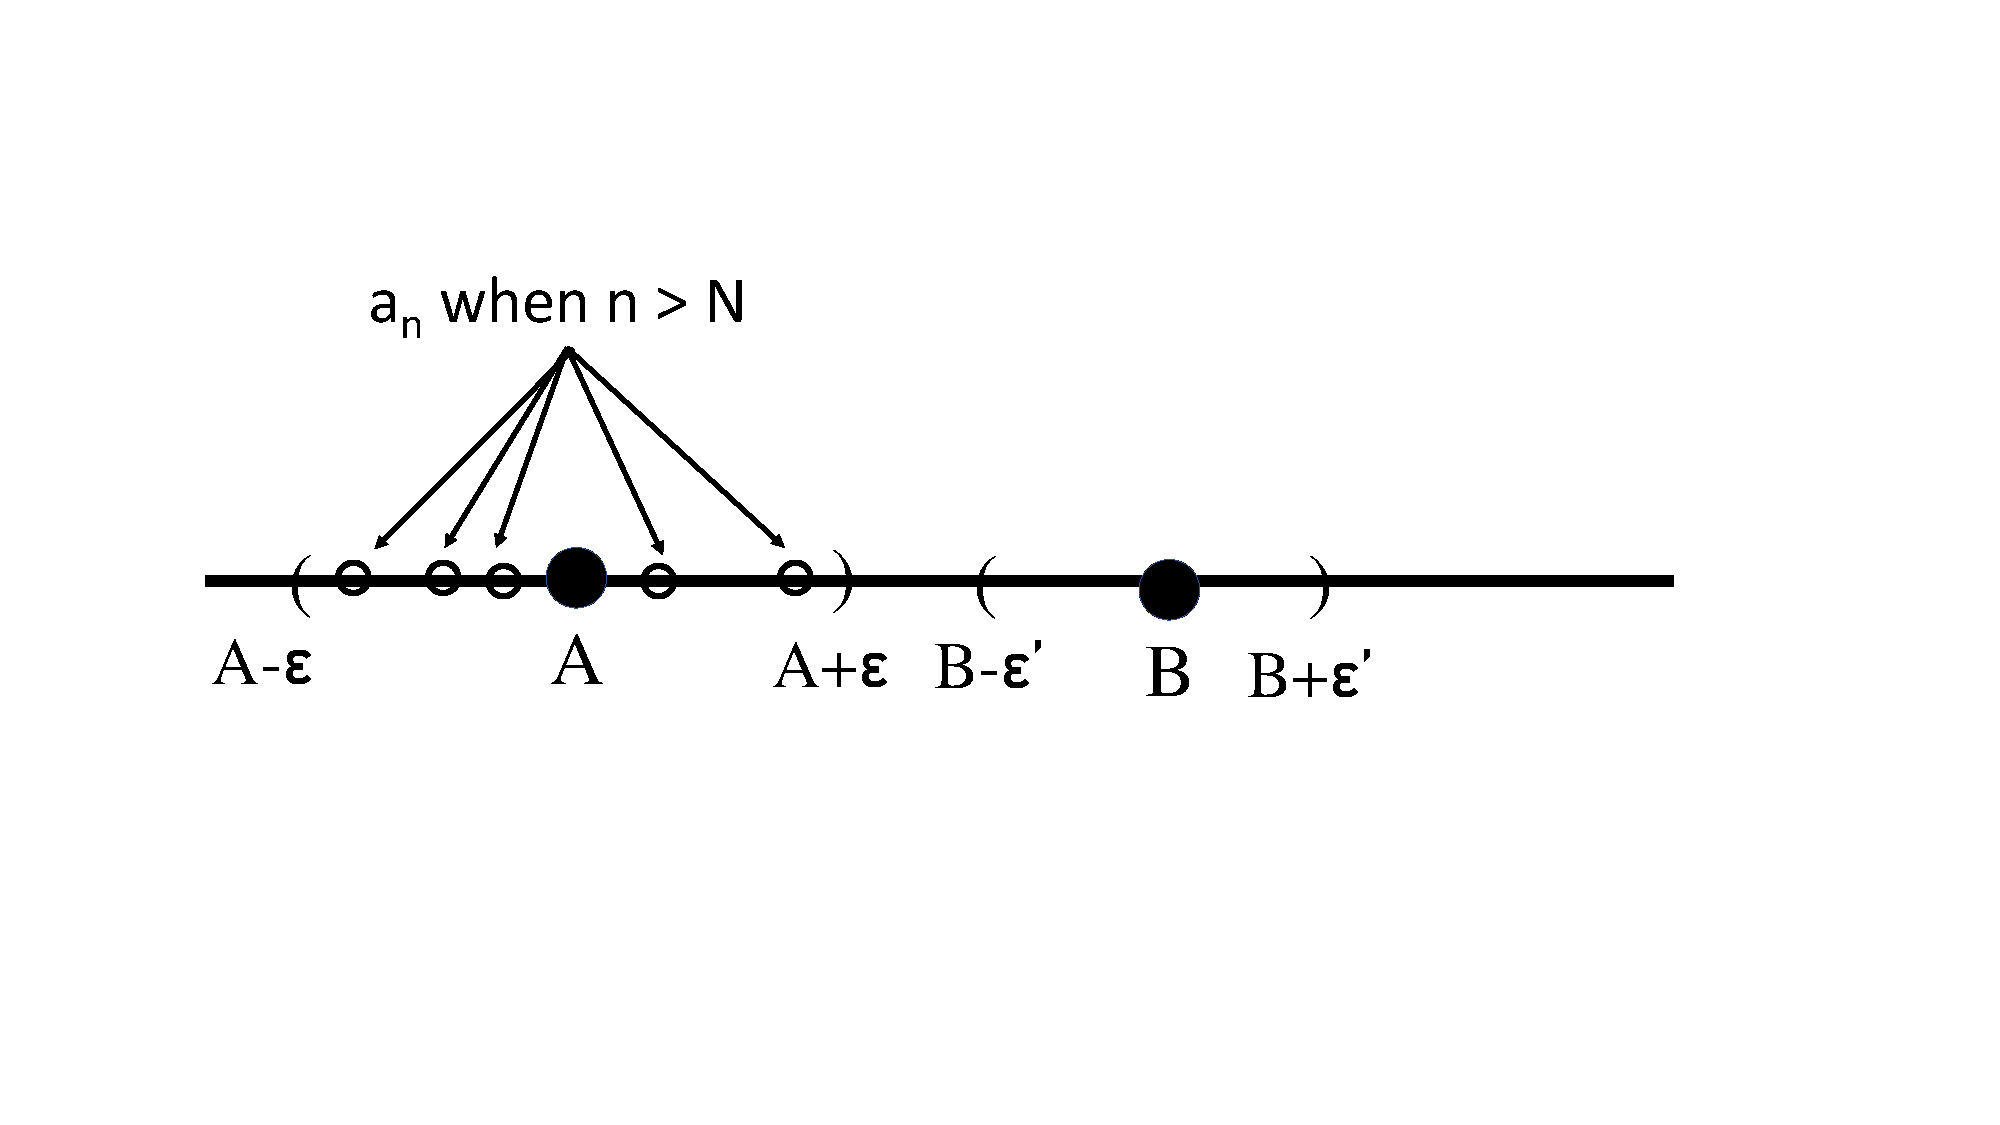
\includegraphics[scale=0.25]{uniqueness}
\end{center}
\caption{Proof of Theorem (\ref{thm:uniqueness})\label{fig:uniqueness}}
\end{figure}

The next theorem, as well as the following exercises, show how we can evaluate complicated limits by breaking them down into smaller parts.
\begin{thm}\label{thm:sumOfLim}
If $a_n,b_n$ are convergent with $\lim a_n=A$ and $\lim b_n=B$ then
\[
\lim (a_n + b_n) = A+B
\]  
\end{thm}
\begin{proof}
The idea here is that if $a_n$ is close to $A$ and $b_n$ is close to $B$ then their sum must be close to $A+B$, see figure \ref{fig:sumOfLim}. What we need to do is to determine how close is close enough to imply
\[
A+B-\varepsilon \leq a_n+b_n \leq A+B + \varepsilon \ .
\]
Whatever $\varepsilon>0$ may be, there will exist $\varepsilon_1>0, \varepsilon_2>0$ such that $\varepsilon_1 + \varepsilon_2 < \varepsilon$, and we have (by assumption) $N_1,N_2$ for which
\begin{align*}
A-\varepsilon_1 \leq a_n &\leq A+ \varepsilon_1 \ \mbox{ if } n > N_1\\
B-\varepsilon_2 \leq b_n &\leq B+ \varepsilon_2 \ \mbox{ if } n > N_2
\end{align*}
thus
\[
A+B-\varepsilon \leq a_n+b_n \leq A+B + \varepsilon \ .
\]
if $n$ is greater than both $N_1$ and $N_2$.

\end{proof}
\begin{figure}
\begin{center}
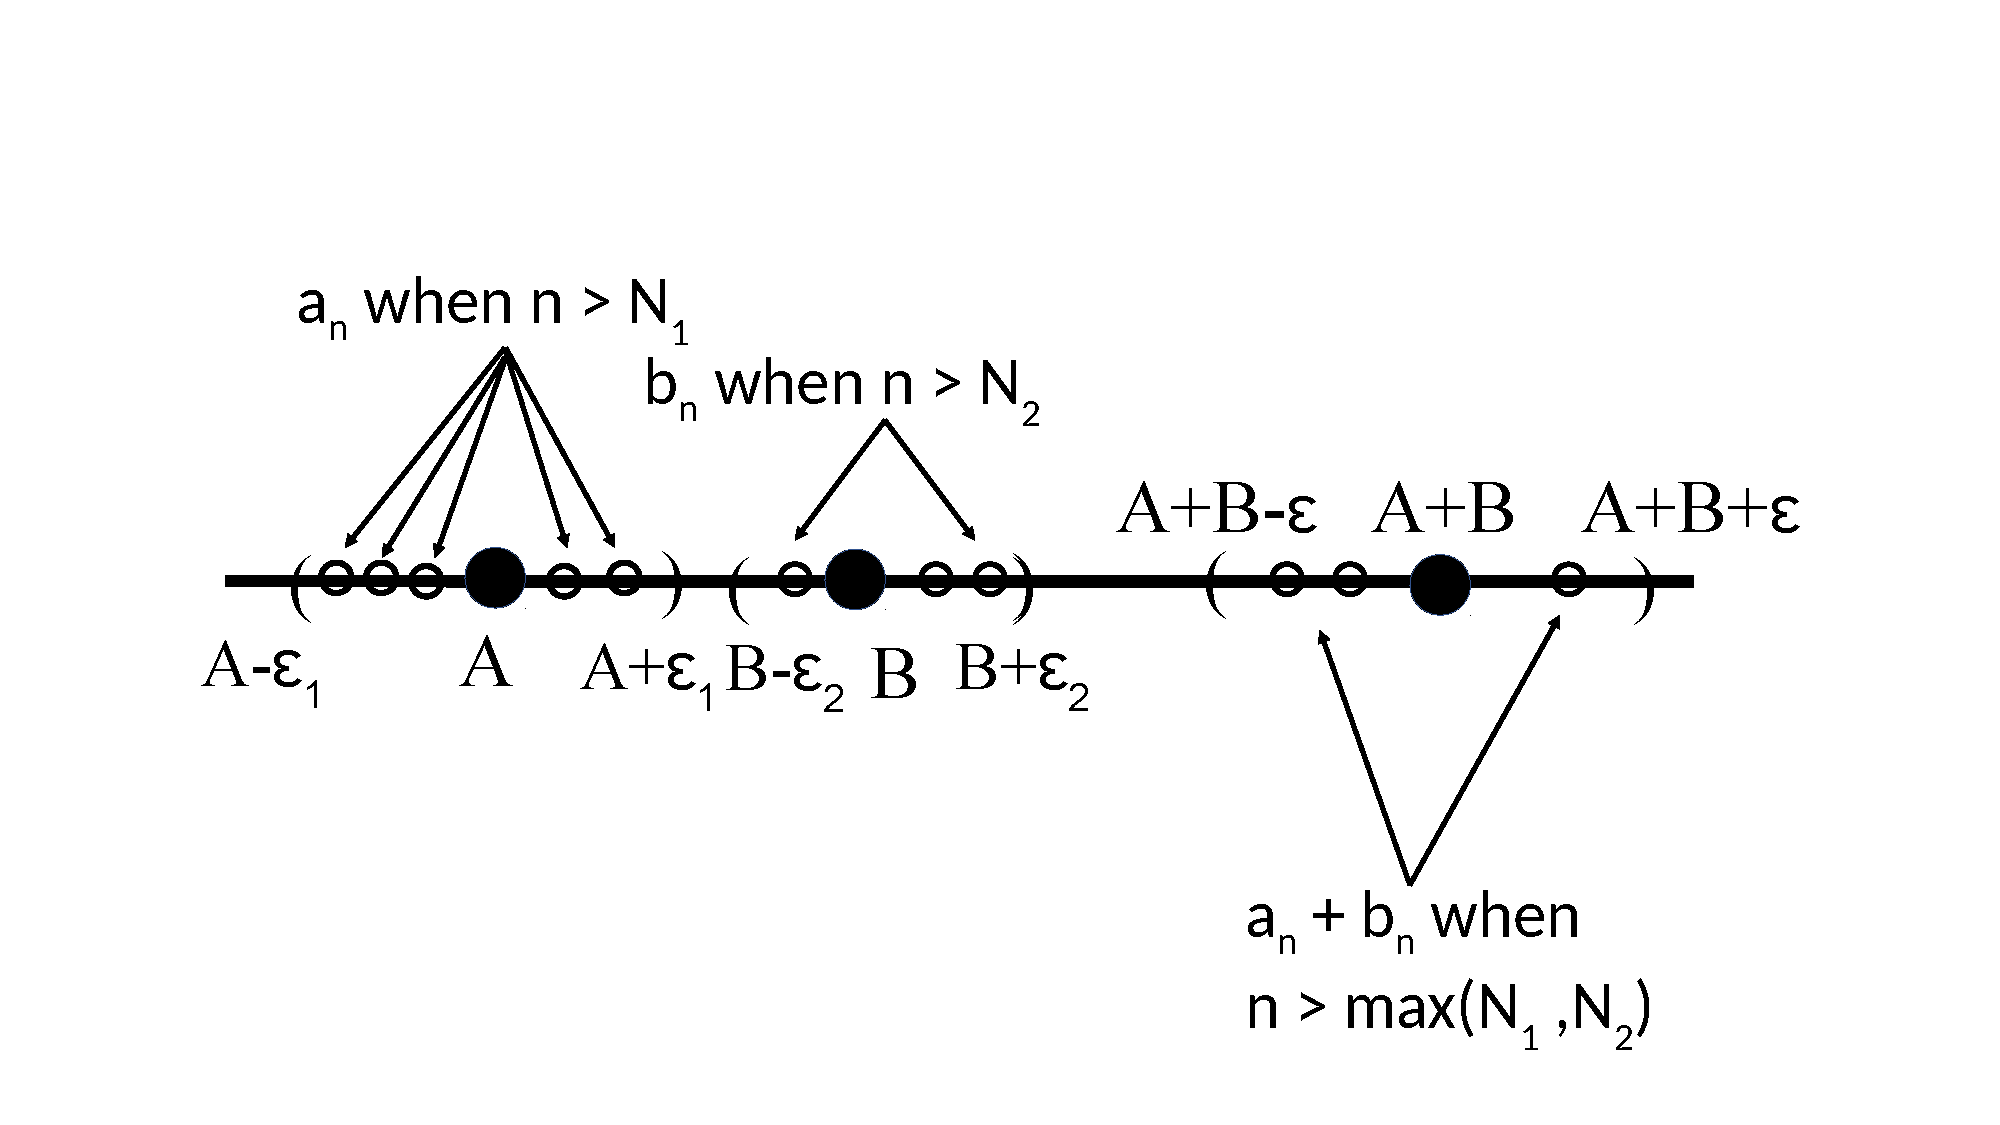
\includegraphics[scale=0.25]{sumOfLimits}
\end{center}
\caption{Proof of Theorem (\ref{thm:sumOfLim})\label{fig:sumOfLim}}
\end{figure}

In addition to manipulating sequences by performing algebraic operations on their terms, we can also ``thin out" a sequence by dropping some terms. The next theorem tells us that if $a_n$ converges, then sequences like $a_2,a_4,a_6,a_8\cdots$ also converge to the same limit.
\begin{thm}\label{thm:arithmeticSubsequenceLim}
If $\lim a_n$ exists and $r,s$ are integers with $r>0$ and $b_n=a_{rn+s}$ then
\[
\lim b_n = \lim a_n
\]
\begin{proof}
Let $\alpha=\lim a_n$. Given $\varepsilon$, take $N$ such that $n>N$ implies $|a_n-\alpha|<\varepsilon$. Then $m > \frac{N-s}{r}$ implies $rm+s>N$ and thus $|b_m-\alpha|<\varepsilon$
\end{proof}
\end{thm}
An important special case is when $r=1, s>0$; then $b_n$ is the sequence $a_s, a_{s+1}, a_{s+2}\cdots$. We call such a sequence a \emph{tail} of $a$. Any tail of a sequence determines its limit.%\footnote{We can take advantage of this to let ourselves be a bit careless about writing things like $\lim 1/a_n$; there may be some $n$ such that $a_n=0$ so $1/a_n$ is undefined, but if $\lim a_n \neq 0$ then, when $n$ is large enough, we must have $a_n \neq 0$. }
In fact a considerably more general statement is true and left as an exercise (theorem \ref{thm:subsequenceLim}).


\subsection{Exercises}\label{sec:limitTheorems}
Prove the following.  These can be proved in a manner similar to our proof of theorem \ref{thm:sumOfLim}.

\begin{thm}\label{thm:equalLim}
If $\lim a_n = \alpha$ and $b_n$ is any sequence such that $a_n-b_n$ converges to zero, then $b_n$ is convergent with $\lim b_n = \alpha$
\end{thm}

\begin{thm}\label{thm:prodOfLim}
If $\lim a_n$ and $\lim b_n$ both exist then 
\[
\lim (a_nb_n) = (\lim a_n) (\lim b_n)
\]  
\end{thm}

\begin{thm}\label{thm:invOfLim}
If all $a_n \neq 0$ and $\lim a_n \neq 0$ then
\[
\lim (1/a_n) = 1/\lim a_n
\]  
\end{thm}

\begin{thm}\label{thm:ineqLim}
If $a_n \leq b_n$ for all $n$ and both limits exist then
\[
\lim a_n \leq \lim b_n
\]  
\end{thm}
Is it possible to have $a_n < b_n$ for all $n$ and yet $\lim a_n = \lim b_n$?

\begin{thm}\label{thm:constTimesLim}
For any constant $c$, if $\lim a_n$ exists then
\[
\lim (ca_n) = c\lim a_n
\]  
\end{thm}

A \emph{subsequence} of a sequence is a sequence obtained by dropping some elements and keeping others, preserving the original order. More formally, if $n_i$ is a sequence of integers such that $n_0 < n_1 < n_2 \cdots$ then $b_n = a_{n_i}$ is a subsequence of $a_n$. Prove:
\begin{thm}\label{thm:subsequenceLim}
If $b_n$ is a subsequence of a convergent $a_n$, then $\lim b_n = \lim a_n$.
\end{thm}


Find the limits of the following, or show non-convergence:
\begin{enumerate}
\item $a_n = \sqrt{n+1}$
\item $a_n = \frac{(-1)^n}{n}$
\item $a_n = \lceil 1 + \frac{(-1)^n}{n} \rceil$ Here $\lceil\rceil$ is the \emph{ceiling} function which ``rounds up" fractions to the next larger integer; so  $\lceil7\rceil=7$,  $\lceil7.00001\rceil=8$, $\lceil7.9\rceil=8$ et cetera.
\end{enumerate}



\subsection{The Meaning of Limits}\label{sec:MeaningOfLimits}
We now have developed some tools for calculating limits and have determined $\lim a_n$ for various sequences. At this point it would be fair to ask why we are interested in such problems. Determining the limit of a sequence can be an interesting puzzle, but there is much more to it. We have already seen that this concept lets us give an unambiguous meaning to infinite decimals like $\frac{1}{3}=0.33\cdots$; more generally, limits are important when we can show that $\lim a_n$ is in fact equal to some other, ``independently meaningful" thing that can be described without reference to the sequence $a_n$ but which is difficult (or impossible) to handle directly. 

Consider for instance theorem (\ref{thm:prodOfLim}), and consider what happens if $a_n = b_n$. Then the theorem tells us that, if $r_n$ is  a convergent sequence with $\lim r_n^2 = 2$, we must have $\lim r_n = \sqrt{2}$. And if we want to know $\sqrt{2}$ out to three decimal places, we know there will be \emph{some} $N$ such that $|r_N - \sqrt{2}| < 10^{-3}$, so $r_N$ is a sufficient approximation. If we can determine what this $N$ is, we can compute the desired approximation.\footnote{This is more than just a theoretical possibility; it is the basic idea for how computers come up with answers like 0.7986355100472928 when we evaluate expressions like $cos(37^\circ)$.}

How can we find such a sequence? Around 1500 B.C. Babylonian mathematicians found a way, given any positive $X$, to cook up a sequence whose limit would be $\sqrt{X}$.\footnote{They did not state their results in these terms, but the idea was the same.} Start with $r_0 = X$ and define
\begin{equation}\label{eq:sqRootApprox}
r_n = \frac{1}{2}(r_{n-1} + \frac{X}{r_{n-1}})
\end{equation}
Why should we think this will converge to the square root? Supposing for now that $X>1$ (the other case is similar), we have started with a value  $r_0 = X$ which is certainly larger than $\sqrt{X}$; but if $r_{n-1} > \sqrt{X}$ then
\[
\frac{X}{r_{n-1}} < \frac{X}{\sqrt{X}} = \sqrt{X}
\]
and similarly whenever $r_{n-1} < \sqrt{X}$ we get $\frac{X}{r_{n-1}} > \sqrt{X}$.
So the hope is to get a better approximation by taking the average of something that is too large and something that is too small.
Now we will show that this clever idea actually works!  We need to show that $\lim r_n^2 = X$. If $r_n^2$ is convergent then
\begin{equation}\label{eq:sqRootApproxExercise}
\lim r_n^2 = \lim \frac{1}{4}(r_{n-1} + \frac{X}{r_{n-1}})^2
\end{equation}
We leave this as an exercise: supposing $\lim r_n^2 = L$, use (\ref{eq:sqRootApproxExercise}) and the previous exercises to set up an equation for $L$ and solve it to get $L=X$.

But is the sequence $r_n$ in fact convergent? Yes; if $|r_n^2 - X| < \varepsilon$, then $|r_n-\sqrt{X}|$ can be no larger than $2\sqrt{\varepsilon}$. We do not have to worry about the negative square root since $r_n$ is always positive.%We claim that $r_n$ is always an overestimate of the square root and that $r_n$ is strictly decreasing.

How quickly does $r_n$ approach the square root? We must consider that question if we hope to use some particular $r_n$ as an approximate value with known accuracy. We leave it as an exercise to show that
\[
r_n^2 - X < (r_{n-1}^2 - X)/2
\]
It then follows by induction that
\[
|r_n^2 - X| < \frac{r_0^2-X}{2^n} = \frac{X^2-X}{2^n}\ .
\]
Thus each iteration at least cuts the error in half; this means we can get a rather accurate approximation with a modest number of iterations.

By the way, one might note that we can easily get a sequence that converges to $\sqrt{X}$, say by just letting $a_n = \sqrt{X}$ for all $n$! But our vague sense that this is somehow ``cheating" is entirely correct. To have something useful we need terms that we can actually compute. When a number is given as $a/b$ for explicit integers $a,b$, we have some confidence that we could (if needed) pour $a/b$ liters of liquid into a tank, cut a length of $a/b$ meters from a longer wire and so on; we can also compare $a/b$ to another $a'/b'$ to determine which is larger, and can add or multiply two such quantities to get an equally explicit result. None of that is possible with only a verbal description like ``the quantity which, when multiplied by itself, yields 2". 


\subsubsection{Exercise}
Write a computer program to implement the Babylonian algorithm. Compare your results to what you get from software like Sage, Matlab, Mathematica et cetera.


\subsection{Irrational Numbers}\label{sec:sqrtIrrational}
We have on a couple of occasions declared that no fraction -- i.e. no expression of the form $a/b$ with $a,b$ both integers -- can be equal to $\sqrt{2}$. Suppose there were such a fraction, and assume it is written in lowest terms, i.e. $a$ and $b$ have no common factor. By definition we must have
\[
(a/b)^2 = a^2/b^2 =2
\]
Thus $a^2 = 2b^2$. This means that $a^2$ is even, so $a$ is even; we can write $a=2\hat{a}$ and $\hat{a}$ is still an integer. But then
\[
a^2 = 4\hat{a}^2 = 2b^2
\]
so $b^2 = 2\hat{a}^2$, thus $b$ must also be even. This makes no sense, since the fraction is in lowest terms.

Fractions of integers are called ``rational" numbers (since they are \emph{ratios} of integers); other numbers are thus called ``irrational", which is perhaps an unfortunate choice of words! The only integers with rational square roots are the perfect squares $(0,1,4,9,16,24,\cdots)$, i.e. integers of the form $m=n^2$, whose square roots are integers; and the analagous statements hold for cube roots et cetera. This is a fundamental fact, and not too hard to prove (by generalizing what we just did for $\sqrt{2}$); see appendix (TBD).

It is also the case that $\pi$ is irrational, but this fact is very much harder to prove, in part because the geometric property ``ratio of circumference to diameter" does not immediately give us an algebraic expression we can manipulate. The irrationality of $\pi$ is not essential for the topics we cover here, so we will not attempt a proof.

We do note here that rational and irrational numbers are packed together tightly and thoroughly mixed on the number line:

\begin{thm}
Every non-empty open interval $(a,b)$ contains both rational and irrational numbers.
\end{thm}
\begin{proof}
Use Archimedean property; some integer $N$ has $1/N < b-a$, so something of the form $k/N$ is in the interval, then use exercises to get irrational number very close to $k/N$.
\end{proof}


\subsubsection{Exercises}
Prove:
\begin{enumerate}
\item The square root of 5 is irrational.
\item The cube root of 2 is irrational
\item The sum of a rational number and an irrational number is irrational.
\item The product of a non-zero rational number and an irrational number is irrational.
\end{enumerate}


\subsection{A Note on Notation}
So far we have always had $n$ as the index of our sequences, but a complicated expression might involve many variables. When we need to make everything more explicit, we will write things like
\[
\lim_{n \to \infty}(ca_{rn+s}) = c\lim_{n \to \infty} a_n
\]
to show that $n$ is the variable going to infinity while $c,r$ and $s$ are constants.


%\subsection{Another Note on Notation}
%Discuss ``austere" notation $\lim a$ since $a$ with no subscript is the sequence itself. Will not use it much but it is useful when we have multiple indices, as in the subsequence theorem.


\subsection{Limits Equal to Infinity}
Both $a_n = (-1)^n$ and $b_n=2^n$ are divergent, but in some sense $b_n$ is a more reasonable-looking sequence; while $a_n$ indecisively bounces around, $b_n$ is at least going somewhere: to infinity! And in fact we can write $\lim b_n = \infty$, extending definition (\ref{def:limit}): 
\begin{defn}\label{def:limitEqInfty}
Let $a_n$ be a sequence of real numbers. If,
for every $M > 0$, there exists an integer $N_M$ such that
\[
a_n > M
\]
whenever $n \geq N_M$ we write
\[
\lim a_n = \infty
\]
\end{defn}
Comparing to definition (\ref{def:limit}), we have replaced the assertion that $a_n$ eventually becomes``close to $A$" with the assertion that $a_n$ eventually becomes ``large"; the limit exists if this remains true no matter how small our threshold for close (or how big our threshold for large) may be.

We also write $\lim a_n = -\infty$ if for every $M<0$ we have $a_n < M$ when $n$ is sufficiently large. Note that this is equivalent to $\lim -a_n = \infty$. When we write something like $\lim a_n > 0$, we include the possibility of  $\lim a_n = \infty$. We even can write $\lim a_n < \infty$ to mean that the limit is real or $-\infty$.

Traditionally we say that a sequence with an infinite limit ``diverges to infinity", rather than saying it converges.

The results from section (\ref{sec:limitTheorems}) have appealing analogues for infinite limits; we prove some of these and leave the rest as exercises.

\begin{thm}\label{thm:prodOfInfLim}
If $\lim a_n > -\infty$ and $\lim b_n = \infty$ then
\[
\lim (a_n+b_n) = \infty
\]  
and if $\lim a_n > 0$
\[
\lim (a_nb_n) = \infty
\]  
\end{thm}
\begin{proof}
Let $\lim a_n=\alpha$. The idea of the first equation is that eventually $a_n$ is almost just $\alpha$, and even if $\alpha$ is something like $-10^{10000}$, adding this finite quantity to $b_n$ will not stop us from reaching infinity. Given $M>0$, take $N$ large enough that both
\begin{itemize}
\item $a_n > \alpha-1$ (of course by definition we can get $a_n$ in the interval $(\alpha-1, \alpha+1)$, but we do not need the upper bound. What should we do if $\alpha=\infty$?)
\item $b_n > M - (\alpha-1)$
\end{itemize}
We have seen this kind of thing before; we set $N$ to the larger of the two numbers needed to make each requirement hold. Thus when $n>N$ we have $a_n+b_n > M$.
\end{proof}


\begin{thm}\label{thm:invOfInfLim}
If $\lim a_n = \pm\infty$ then
\[
\lim (1/a_n) = 0
\]
If $\lim a_n = 0$ and $a_n > 0$ for all $n$ then
\[
\lim (1/a_n) = \infty
\]
\end{thm}


\begin{thm}\label{thm:ineqInfLim}
If $a_n \leq b_n$ for all $n$ and $\lim a_n = \infty$ then
\[
\lim b_n = \infty
\]  
\end{thm}

\begin{thm}\label{thm:subsequenceInfLim}
If $\lim a_n = \infty$ and $\hat a$ is a subsequence of $a$ then
\[
\lim (\hat a) = \infty
\]
\end{thm}

On the other hand, some combinations are ``indeterminate". Let $I_n$ denote a sequence with $\lim I_n = \infty$, and $Z_n$ denote a sequence with $\lim Z_n = 0$. Then all of the following are possible:
\begin{itemize}
\item $\lim I_nZ_n = \infty$
\item $\lim I_nZ_n = r$ for any real number $r$
\item $\lim I_nZ_n$ does not exist
\end{itemize}
We get the first case from things like $I_n=n, Z_n = \frac{1}{n^2}$, so $I_nZ_n = \frac{1}{n}$; the second case could be for instance $I_n=n, Z_n = \frac{1}{n}$, so $I_nZ_n = 1$. Can you come up with a case for $r=0$?

Similarly let $J_n$ also denote a sequence approaching infinity, we can have $\lim (I_n-J_n)$ be infinity, any real number, or it may not exist; with $I_n = n^2$ consider $J_n = n^2$ or $J_n=n$ or $J_n = n^2 + (-1)^n$.

The expression $\lim \frac{I_n}{J_n}$ is similarly indeterminate. And if $\lim Z'_n=0$, we can could have any value (including infinity or divergence) for $\lim  \frac{Z_n}{Z'_n}$ -- leaving it to the reader's imagination to come up with examples.

The final theorem of this chapter generalizes theorem \ref{thm:oneOverN}, and also makes use of the Archimedean property.

\begin{thm}\label{thm:geometricLim}
For any real number $x$ such that $0 \leq x < 1$
\[
\lim x^n = 0
\]
For any real number $x > 1$
\[
\lim x^n = \infty
\]
\end{thm}
\begin{proof}
Note that either assertion implies the other, by using theorem \ref{thm:invOfInfLim} and replacing $x$ by $x^{-1}$. No prizes for figuring out the case $x=1$.

If $x \leq 1/2$, the first part follows immediately from the Archimedean property; we have $x^n \leq 2^{-n} \leq 1/n$, and leave it to the reader to fill in the details along the lines of the theorem \ref{thm:oneOverN}. Similarly if $x \geq 2$ we immediately have $x^n > n$ and so we go to infinity.
But when $x$ is barely less than (greater than) 1, it is no longer quite so obvious that we can get $x^n$ to be small (large); maybe we will hit a plateau somewhere?
It is never a bad idea to try some numerical experimentation; with $x=0.99999$ or  $x=1.00001$ we have
\begin{equation*}\begin{array}{cccccc}
(0.99999)^{100} &=& 0.9990004948383437 &(1.00001)^{100} &=& 1.0010004951617457\\
(0.99999)^{1000} &=& 0.9900497842463927 &(1.00001)^{1000} &=& 1.010050116582064\\
(0.99999)^{10000} &=& 0.9048369656147593 &(1.00001)^{10000} &=& 1.1051703654947347
\end{array}\end{equation*}
and perhaps we are beginning to have doubts? But going onward
\begin{equation*}\begin{array}{cccccc}
(0.99999)^{100000} &=& 0.3678776017682465 & (1.00001)^{100000} &=& 2.7182682371922975\\
(0.99999)^{1000000} &=& 0.000045397659809679 & (1.00001)^{1000000} &=& 22025.364507834245
\end{array}\end{equation*}
and our faith is restored.
%Indeed we could have stopped with an exponent of 100000, since this is less than $1/2$ so we know that $(0.99999)^{100000n} < 2^{-n}$.

Still we need to prove that the exponent required to get $x^n<\varepsilon$ or $x^n>M$ will not somehow reach infinity before $x$ reaches 1. It is easier to tackle the case $x>1$ directly.
We consider the difference between consecutive values in the sequence:
\[
x^{n+1}-x^n = x(x^n-x^{n-1})
\]
since $x>1$, we can conclude that
\[
x^{n+1}-x^n > x^n-x^{n-1}
\]
So not only do the terms of the sequence increase, but the gap between consecutive terms keeps increasing. Letting $x=1+\kappa$ (so $\kappa>0$) we have $x^1-x^0=\kappa$ and every subsequent gap is greater than $\kappa$. Therefore $x^n > 1 + \kappa n$. For any $M$ we get $x^n>M$ if $n>M/\kappa$, invoking the Archimedean property for the existence of such $n$.
\end{proof}

\subsubsection{Exercises}
\begin{itemize}
\item What happens to $\lim x^n$ for negative $x$?
\item What is $\lim nx^n$ for $0 < x < 1$?
\end{itemize}


\pagebreak
\section{Infinite Series}
\subsection{Geometric Series}
In the first chapter, consideration of $\frac{1}{3}=0.333\cdots$ led us to the sequence
\[
a_n  = \frac{3}{10} + \frac{3}{100} + \cdots + \frac{3}{10^{n-1}} + \frac{3}{10^n}
\]
i.e. defining $a_n$ as the sum of the first $n$ terms of another sequence, here $b_k=\frac{3}{10^k}$.  We now fulfill our promise that we would see other sequences defined in this way.
So we introduce some notation for sequences defined by ever-longer sums.
\begin{defn}\label{def:infSer}
Given any sequence $b_n$ we define the \emph{infinite series}
\[
\sum_{k=0}^{\infty} b_k
\]
to mean
\[
\lim_{n \to \infty} b_0+b_1+b_2+ \cdots + b_n
\]
if the limit exists (in which case we say the series is convergent). Sums of the form $\sum_{k=0}^{n} b_k = b_0+b_1+b_2+ \cdots + b_n$ are called \emph{partial sums} of the infinite series.
\end{defn}

The most fundamental example of a convergent series is known as the \emph{geometric series}: 
\begin{thm}\label{thm:geometricSeries}
For any $-1<x<1$,
\[
\sum_{k=0}^{\infty} x^k = 1 + x + x^2 + \cdots = \frac{1}{1-x}
\]
\end{thm}
\begin{proof}
Before proving the theorem, note that with $x=\frac{1}{10}$ it becomes
\[1.1111\cdots = \frac{10}{9}\]
which is just a mild tweaking of the classic $0.333\cdots = \frac{1}{3}$.

We both demonstrate that the series converges and determine its value by finding an explicit expression for the $k^{\mbox{th}}$ partial sum
\[
a_k(x) = 1 + x + x^2 + \cdots + x^k
\]
The trick is to note how nicely this expression can be manipulated into variations of itself. In particular, multiplying by $x$ only changes the first and last terms: $xa_k(x) = a_k(x) - 1 + x^{k+1}$, thus
\[
a_k(x) = \frac{1-x^{k+1}}{1-x}
\]
and the result follows from theorem \ref{thm:geometricLim}, which tells us that $\lim x^k = 0$.
\end{proof}

It is sometimes convenient to drop the $k=0$ term (which is not very interesting since it is always 1 regardless of $x$) and write
\[
\sum_{k=1}^{\infty} x^k = x + x^2 + x^3 +\cdots = \frac{1}{1-x} - 1 = \frac{x}{1-x}
\]
A noteworthy  special case is $x=1/2$, i.e.
\begin{equation}\label{eq:Zeno}
\sum_{k=1}^{\infty} 2^{-k} = \frac{1}{2} + \frac{1}{4} + \frac{1}{8} + \cdots =1
\end{equation}
which can be visualized as in diagram (\ref{fig:zeno}).
We imagine starting with an empty square of side one, and each term of the series fills in half of what remains. This is a version of the old philosophical puzzle known as ``Zeno's paradox": it should be impossible to ever walk all the way across a room, because before you can get there you first need to get halfway across, then you still need to get halfway from there to your destination, then ... !? The solution to the paradox is that walking across a room does involve an infinite number of shorter walks, but the ever-decreasing durations of these walks are a convergent series, summing to a finite amount of time.
\begin{figure}
\begin{center}
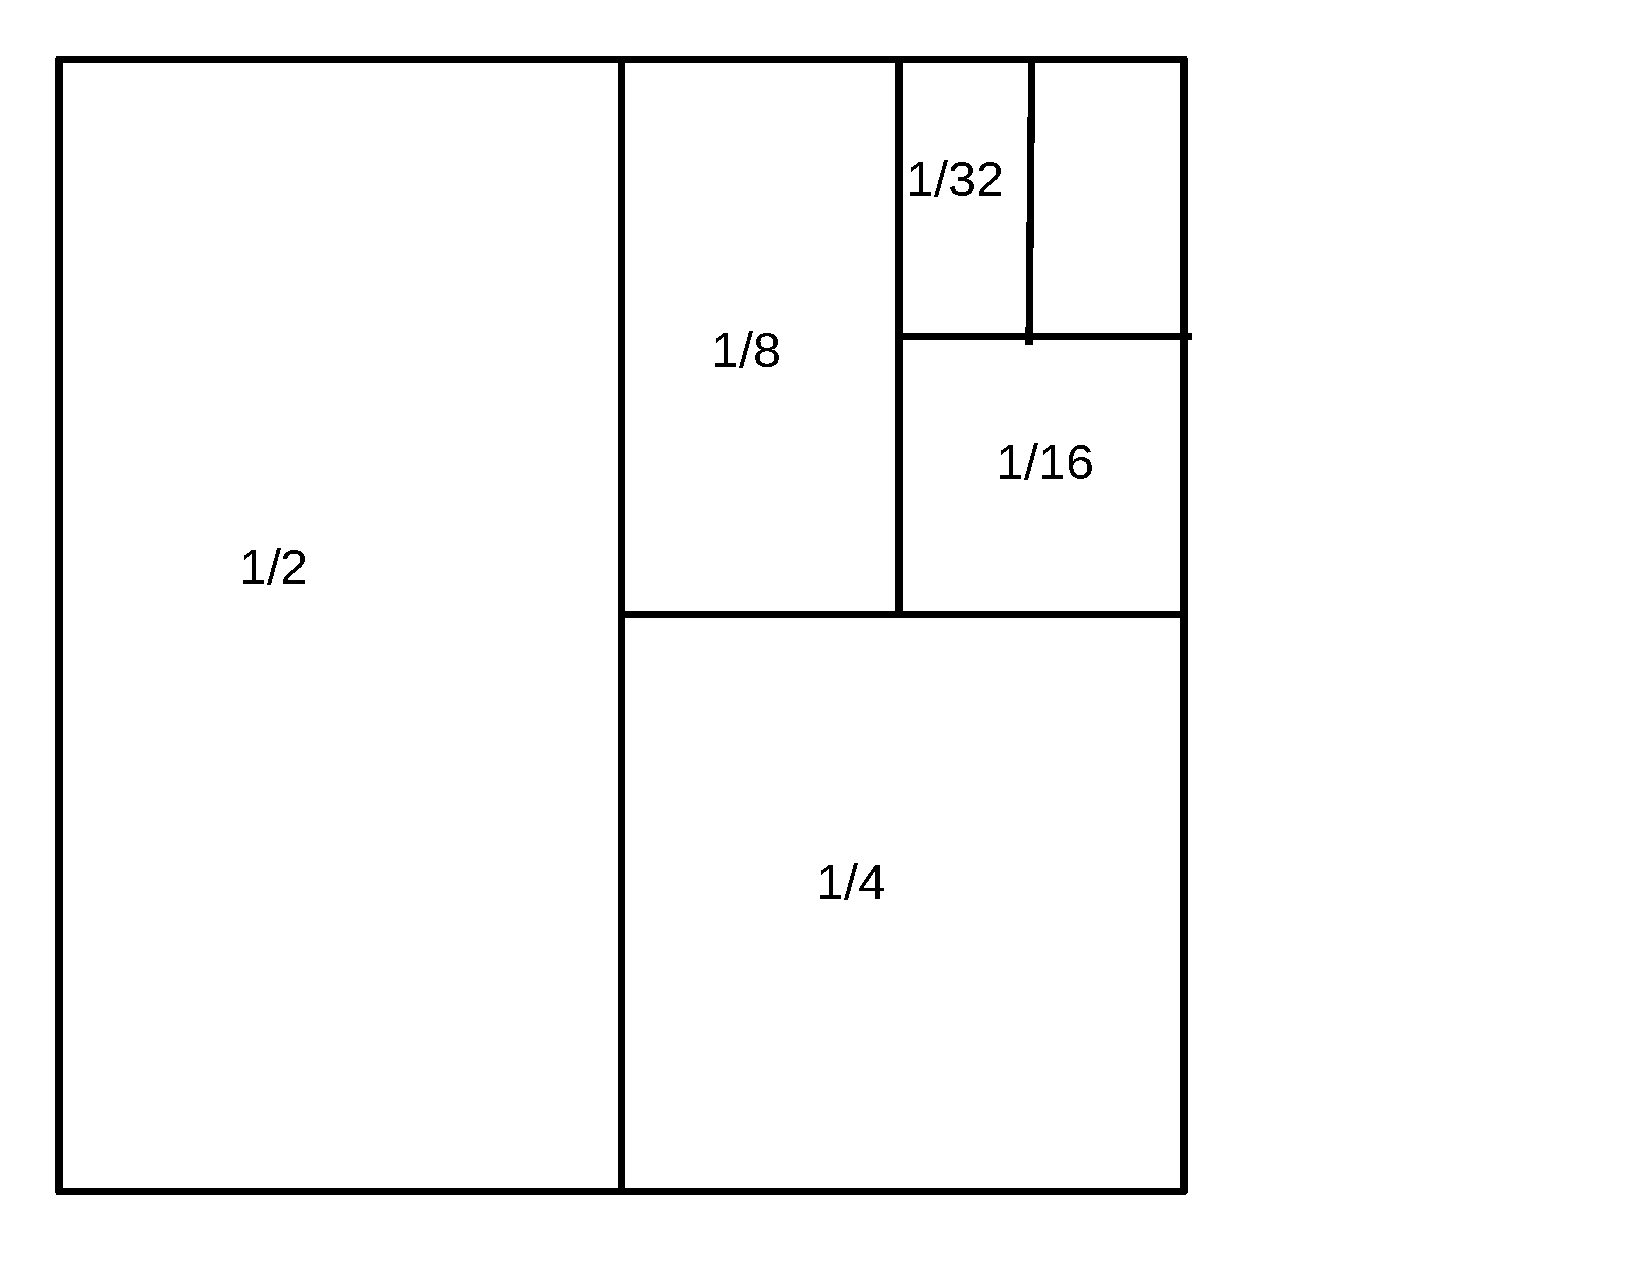
\includegraphics[scale=0.33]{zeno}
\end{center}
\caption{$\sum_{k=1}^{\infty} 2^{-k} = \frac{1}{2} + \frac{1}{4} + \frac{1}{8} + \cdots =1$\label{fig:zeno}}
\end{figure}

\subsubsection{Exercises}
\begin{enumerate}
\item Prove that, if  $\sum_{k=0}^{\infty} b_k$ converges, we must have $\lim b_k = 0$.
\item Evaluate $0.73737373\cdots$ (i.e. express it as a fraction).
\item Prove (assuming convergence) that $c\sum_{k=0}^{\infty} b_k = \sum_{k=0}^{\infty} cb_k$.
\item Evaluate $\sum_{k=0}^{\infty} x^{2k} = 1 + x^2 + x^4 + x^6 + \cdots$ assuming $-1<x<1$.
\item Evaluate $\sum_{k=0}^{\infty} kx^k = x + 2x^2 + 3x^3 + \cdots$ assuming $-1<x<1$. (You cannot get this directly from theorem \ref{thm:geometricSeries}, you will need to work out an expression for the partial sums)
\item Evaluate $\sum_{k=1}^{\infty} \frac{1}{k(k+1)}$. (Forget about theorem \ref{thm:geometricSeries}, just find an expression for the partial sums)
\item The sum (\ref{eq:Zeno}) has an interesting interpretation in terms of probability. If we repeatedly flip a fair coin, what is the probability that we will eventually get ``heads"? One-half is the chance of getting heads immediately, $1/4$ is  the probability of tails then heads, and $2^{-k}$ is the probability that heads first appears at the $k^{\mbox{th}}$ flip: the sum tells us that the probability of eventually seeing heads, if we can flip an unlimited number of times, is one. Does this make sense? By the same reasoning, what is the probability of eventually seeing heads if we repeatedly toss a coin which is biased so that heads appears with probability only $1/3$?
\end{enumerate}

\subsection{Divergent Series}
{\color{red}Harmonic. Exercises on simple variants of harmonic.} 

%At this point what matters is to present more interesting examples of sequences,
%lead this into justification for least-upper-bound assumption, Cauchy sequences (starting with emphasis on sequences with all terms positive).
%But also point out that if we make up some arbitrary rule for $i$th digit, we have (in general) no better description of what the limit is! And if the terms are not of the right form, we might not even be sure we have the decimal digits right ... !?


\subsection{Convergence of Series}
Representation of numbers as decimal expansions is very closely related to convergent series and geometric series.
In fact, an infinite decimal like $\sqrt{2}=1.4142135623730951\cdots$ is nothing but a convenient shorthand for
\begin{equation}\label{eq:decimalExpansion}
\lim_{n\to\infty} 1 + \frac{4}{10} + \frac{1}{100} + \frac{4}{1000} + \frac{2}{10000} + \frac{1}{100000} + \frac{3}{1000000} + \cdots +\frac{d_n}{10^n}
\end{equation}
where $d_n$ is the $n^{\mbox{th}}$ digit. But this raises some surprisingly subtle questions. We always take it for granted that \emph{any} list of digits will define a number -- in the terminology of the previous chapter, we assume that \emph{all sequences of the above form are convergent}. Since we know that many sequences diverge and that it is not always easy to tell, it seems we are assuming quite a lot! But the geometry of the number line makes the assumption thoroughly compelling. We naturally equate ``number" with ``a point on the line"; whenever we add a new digit, we are confining our supposed number/point to an ever-smaller part of the line:
\begin{equation*}\begin{array}{ccc}
1.4 < &\sqrt{2} &< 1.5\\
1.41 < &\sqrt{2} &< 1.42\\
1.414 < &\sqrt{2} &< 1.415
\end{array}\end{equation*}
et cetera. When we ``go to infinity", there is no ambiguity about where this point/number must be. We cannot, say, be left with two candidate points separated by a distance of $10^{-1000}$: after fixing the first 1001 digits, the range of possible values will be narrower than that. Indeed, the boldness of our assumption lies entirely in  the opposite direction, in assuming that the number line is in some sense ``full", so there cannot be a sequence of digits that somehow manages to cut out everything, leaving us with no points at all.

The ``fullness" of the line truly is an assumption, because there is nothing in the rules of arithmetic which requires that an irrational number like $\sqrt{2}$ must exist. There is surely no rule that says every equation must have a solution; if there is no real $x$ such that $x=x+1$ or $x^2=-1$, why must there be something to satisfy $x^2=2$? 
If we were to declare that ``number" means rational number -- i.e. a fraction with integer numerator and denominator -- we would encounter no logical problems at all, since the operations of arithmetic, applied to rational numbers, can only produce other rational numbers.
%If we ``deny the existence" of irrationals, we end up with a vastly smaller collection of convergent sequences -- too small to really be interesting -- but the definition of convergence still makes sense.

Take a careful look at the Babylonian square-root algorithm from section \ref{sec:MeaningOfLimits}: we never actually proved that $X$ has a square root, we only proved that \emph{if} $X$ has a square root, the sequence $r_n$ must converge to it.

Our confidence in the existence of things like $\sqrt{2}$ comes from geometry; the diagonal of a 1-by-1 square can be nothing else. This follows from the Pythagorean theorem -- or more simply from diagram \ref{fig:sqrt2}.  And we cannot limit our geometric intuition to lines; we feel just as strongly that any curve could be ``unrolled" into a line segment, and so must have a numeric length -- hence $\pi$ must be a number because it is the circumference of a circle with diameter $1$.
\begin{figure}
\begin{center}
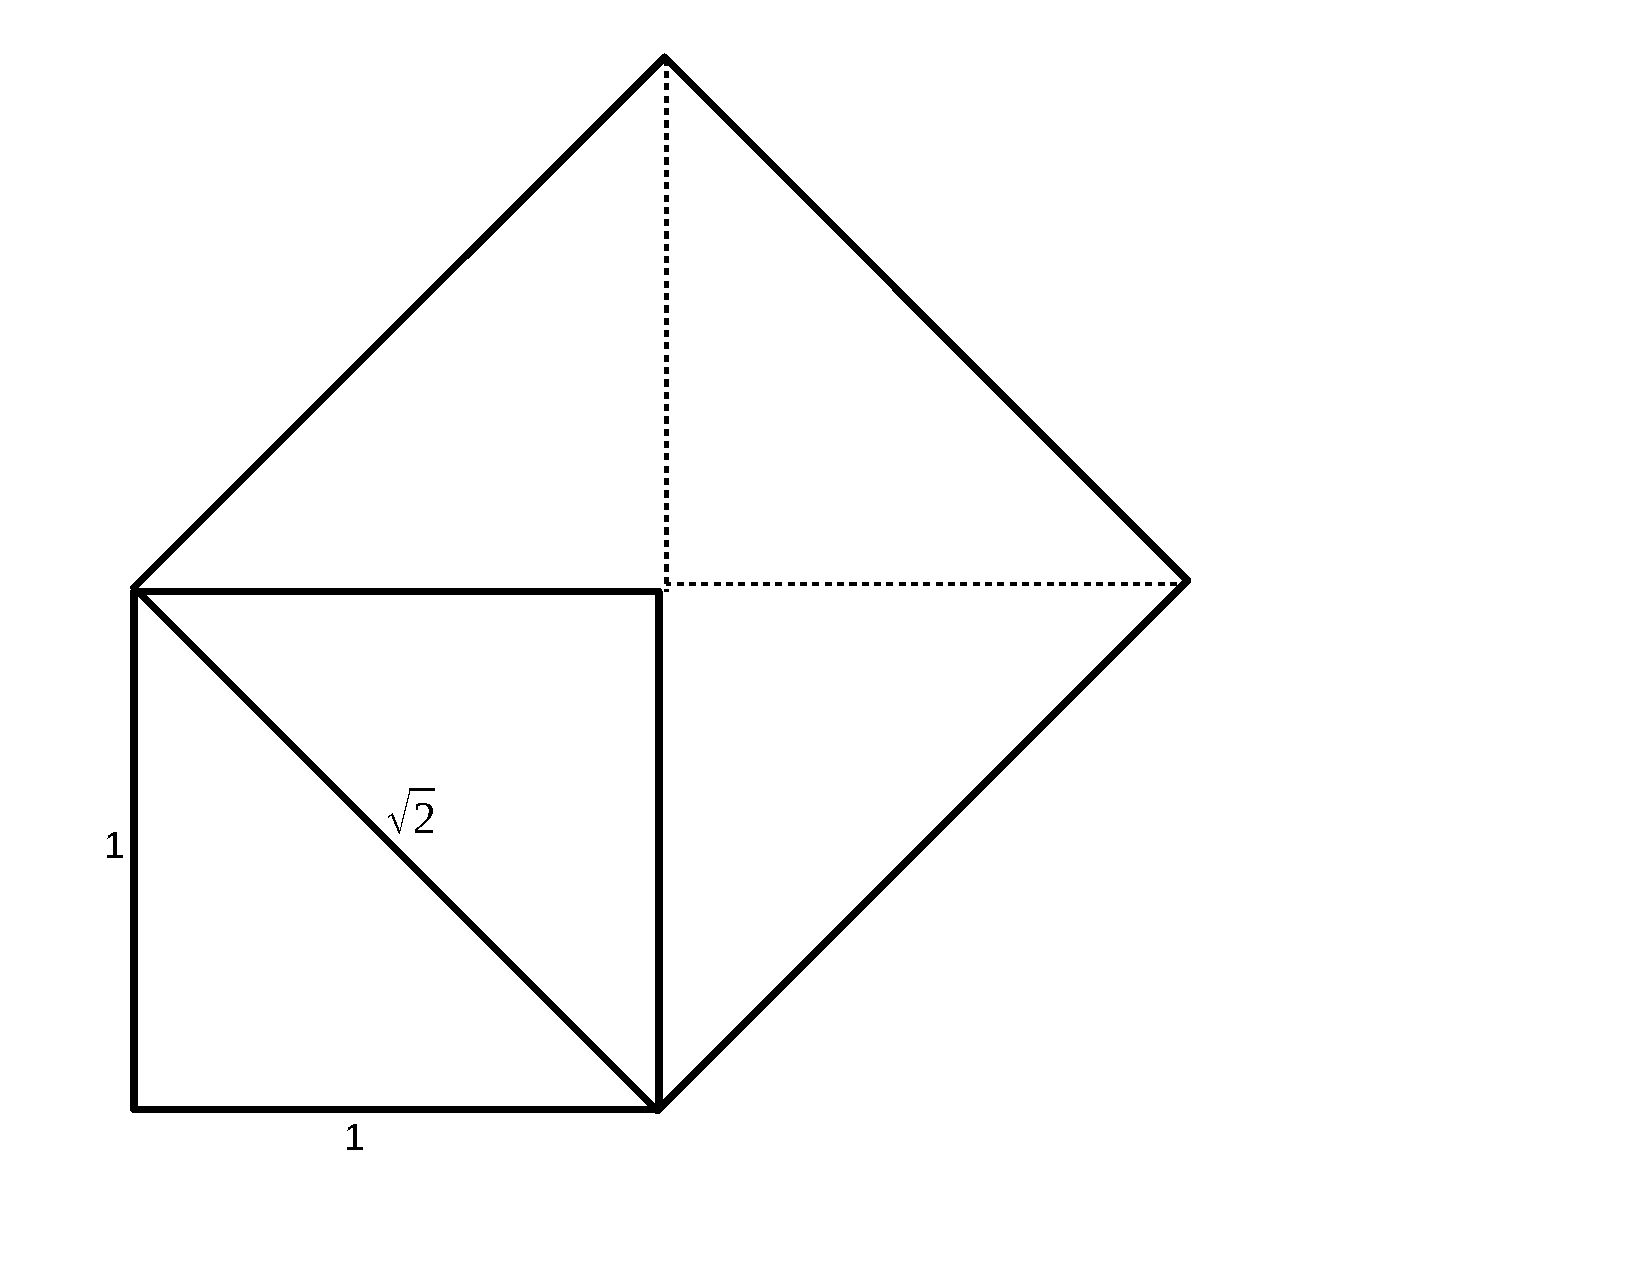
\includegraphics[scale=0.33]{sqrt2}
\end{center}
\caption{Area of the larger square is four triangles, i.e. 2, so its side is the square root of 2\label{fig:sqrt2}}
\end{figure}

We will, in fact, assume that decimal expansions always converge, but we will state that assumption in a rather different form; one which is more useful for proving theorems and which is not tied to the particular notation we use for writing numbers. Before that we must first introduce another central concept of calculus: continuity.
%At that point we will be faced with a rather substantial collection of observations which seem like they must be true, but cannot be proved without assuming the fullness of the number line.
For now we will just prove (as an exercise) a theorem which completely settles which decimals are rational and which are not.
%As in the first chapter, we have begun by focusing on the familiar convention of writing numbers as possibly infinite decimal expansions, but  we actually want to reason about quantities in a way that is not tied to the notation we use to write them. And then we will be done making assumptions; all further results will follow from elementary arithmetic, the Archimedean property, and our to-be-stated assumption about convergence.
%We could in fact \emph{define} a real number to be a sequence of digits; then could define addition/multiplication by giving the rules for how to perform these operations and so on. 

\subsubsection{Exercises}
\begin{enumerate}
\item Prove that if an infinite series of the form
\begin{equation}
\sum_{n=1}^{\infty} \frac{d_n}{10^n}
\end{equation}
converges, the sum must be $<=1$
\item The infinite decimal $0.d_1d_2d_3...$ is  \emph{ultimately periodic} if there are integers $t\geq 0,p\geq 1$ such that $d_{i+p}=d_{i}$ whenever $i>t$; in other words, after an  arbitrary initial segment of length $t$, we keep repeating the same pattern of $p$ digits. Prove that every ultimately periodic decimal represents a rational number.
\item Prove the converse: every rational number has an ultimately periodic decimal representation. (Consider using long division to get one digit after another; what would cause the sequence of digits to become periodic?)
\item Would these two results be any different if we used a base other than ten?
\end{enumerate}


{\color{red}
 \subsection{Convergence Tests}
 Put convergence tests in separate chapter, after derivatives.}
 %Do not need full details of all tests for first draft, but must decide exactly how to formulate Cauchy property and suggest flavor of how this section should look.
%Here is where we have do deal with pure existence of sums we cannot evaluate, so we must make explicit something like the least-upper-bound assumption; given the way we have developed the material, it is better to take convergence of Cauchy sequences as our axiom.
%
%Spivak has the following (skipping the integral test of course): look closely at proofs (exactly where is LUB axiom used?). In place of integral test should be able to manipulate bounds on sum of $x^{-p}$? i.e. approximate the integral; integrals are just expressions for approximate partial sums
%
%\begin{itemize}
%\item comparison (441); this is direct application of LUB; for us it should be the motivation to assume that limits exist even when we cannot evaluate them
%\item ratio (443); this is basically applying comparison test against geometric
%\item Leibniz (448) - again just a careful application of sup/inf/lub et cetera.
%\item product of series (454); might skip this since we have already delayed derivatives so long!
%\end{itemize}


\pagebreak
\section{Continuity}
We have seen several theorems showing that limits ``behave nicely" when we mix them with other operations. All these results are variations on the same theme; when $a_n, b_n$ get close to their limits $\alpha, \beta$, then $a_n+b_n$ is close to $\alpha+\beta$, $a_nb_n$ is close to $\alpha\beta$ and so on. We have not said much about trig functions or logarithms; we expect that the reader has some familiarity with such things, but it takes a fair amount of work just to get a completely precise definition of what these functions are, so we have put them aside for the moment. Nevertheless it makes sense to expect that, when $n$ is large enough, $\sin(a_n)$ will be close to $\sin(\alpha)$ et cetera. This is the way we expect most functions to behave, and it is essential for most uses of mathematics to describe the world, since all measurements are inexact. When we measure the angle between two laser beams or two metal bars, the most we can say that is very close to 47 degrees; we could not make much use of trigonometry  in engineering without some guarantee that the sine of this angle must be close to $\sin(47^\circ)$. We encapsulate this idea with the following (preliminary) definition:

\begin{defn}\label{def:continuityPrelim}
The function $f$ is \emph{continuous} at $\alpha$ if
\[\lim f(a_n) = f(\alpha)\]
for all convergent sequences with $\lim a_n = \alpha$.
\end{defn}

This definition will need a bit of tweaking, but before delving into the technical details one should make sure  to understand that this formal definition sums up the intuitive ideas of the preceding paragraph. Note that we have already implicitly proved a result along the lines of ``most normal-looking functions are continuous":

\begin{thm}\label{thm:ratFunctsCont}
Let $f(x)=\frac{p(x)}{q(x)}$ where $p,q$ are polynomials. Then $f$ is continuous everywhere it is defined (i.e. everywhere that $q(x) \neq 0$).

A function of this form is called a  \emph{rational} function.
\end{thm}
\begin{proof}
Let $p(x) = p_nx^n + \cdots + p_1x + p_0$ and $q(x) = q_mx^m + \cdots + q_1x + q_0$.
Our previous results on sums and products tell us that, if $a_n$ converges to $\alpha$,
\[
\lim p(a_n) = p_n(\lim a_n)^n + \cdots + p_1(\lim a_n) + p_0 = p(\alpha)
\]
and
\[
\lim q(a_n) = q_m(\lim a_n)^m + \cdots + q_1(\lim a_n) + q_0 = q(\alpha)
\]
Since the limits exist, we also already know that, if $q(\alpha)\neq0$, 
\[
\lim f(a_n)=\frac{\lim p(a_n)}{\lim q(a_n)}=f(\alpha)
\]
\end{proof}

The proof of  (\ref{thm:ratFunctsCont}) points toward the tweaks we need. In order for the definition to make any sense, our  $f$ must be defined at $\alpha$; furthermore the only sequences that make sense here are those with values in the domain of $f$, so that each $f(a_n)$ is defined. In fact, we are going to restrict things even more. We are interested in what happens to $f(x)$ as $x$ gets close to $\alpha$, so we want $f$ to be defined at all points ``around" $\alpha$; in other words, $f$ should be defined on an \emph{open interval} containing alpha, leading to

\begin{defn}\label{def:continuity}
The function $f$ is \emph{continuous} at $\alpha$ if it is defined at all points in an open interval $I$ containing $\alpha$ and 
\[\lim f(a_n) = f(\alpha)\]
for all convergent sequences $a_n$ with values in I and $\lim a_n = \alpha$.
\end{defn}
Note that this definition implicitly requires that $f(a_n)$ must be convergent for all such $a_n$. Recall that an open interval $(a,b)$ is the set of all $x$ such that $a < x < b$; since we exclude the endpoints, our interval $I$ must contain points on both sides of $\alpha$.

Recall theorem \ref{thm:subsequenceLim}, which states that $\lim a_n = \alpha$ is determined by any tail subsequence $a_k, a_{k+1} \cdots$. If $I$ is an open interval and $\lim a_n \in I$, We will have $a_n \in I$ when $n$ is large enough (take $\varepsilon$ small enough to get $(\alpha-\varepsilon,\alpha+\varepsilon)$ inside $I$). This means that any convergent sequence approaching $\alpha$ is applicable to the definition of continuity, if we truncate it enough to keep only values that are within the domain of $f$.

Our theorems about the behavior of limits under various operations carry over directly to continuous functions, for instance

\begin{thm}\label{thm:sumOfCont}
If functions $f,g$ are continuous at $\alpha$ then so is $f+g$.
\end{thm}
\begin{proof} Follows almost immediately from results on sequences. \end{proof}

\subsubsection{Exercises}
\begin{itemize}
\item Prove the claim made above that there is a tail of $\{a_n\}$ contained in $I$.
\item Composition, product of continuous functions are continuous. Absolute value is continuous.
\end{itemize}


\subsection{Graphs of Continuous Functions}
Continuity is closely related to our expectation of what the graph of a function should look like. The functions studied in precalculus -- polynomials, trig, square roots et cetera -- have graphs that can be drawn as smooth unbroken curves, ``without lifting the pen from the paper" (in the classic phrase of the pre-computer era); the only exceptions are the few points where these functions are undefined, such as $\frac{1}{x}$ at $x=0$. A function whose graph has a visual break is discontinuous at that point even if it is defined there. A good example is the ceiling function $\lceil x \rceil$ introduced in the last chapter. It is discontinuous at every integer; for instance $\lceil 1 \rceil = 1$, but $\lim \lceil 1 + \frac{1}{n} \rceil = 2$.
%For instance the ``sign" (not sine!) function (see figure \ref{fig:discontinuity})
%\[
%f(x) = \begin{cases}
%1, &x > 0\\
%0, &x = 0\\
%-1, &x < 0
%\end{cases}
%\]
%is discontinuous at zero; any sequence of positive numbers with $\lim a_n = 0$ will have $\lim f(a_n) = 1$. Note that it would be discontinuous no matter how we defined $f(0)$.

A more extreme example would be
\[
f(x) = \begin{cases}
1, &x\  \text{is rational}\\
0, &x\  \text{is irrational}
\end{cases}
\]
which jumps around so much that it cannot be drawn as a curve at all; it is discontinuous everywhere (see exercise ??). 

The most ``well-behaved" functions should be ones that could plausibly represent the motion of a physical object; assuming objects cannot teleport, such motion defines an unbroken curve. Similar considerations apply to other physical quantities: temperature cannot rise from $99$ to $100$ degrees without momentarily passing through each intermediate $99 < y < 100$ et cetera. The definition of continuity is an attempt to capture some of that intuition. We will see in section \ref{sec:behaviorOfContFuncs} that continuous functions can still behave in physically implausible ways, but first we will consider the consequences of this ``intermediate value" property, which, stated more precisely, claims:

\begin{claim}[The Intermediate Value Property]\label{claim:intermediateValue}
Let $f$ be continuous at all points of the closed interval $[a,b]$, with $f(a)<f(b)$. Then for any $f(a) < y' < f(b)$ there exists $a < x' < b$ such that $f(x') = y'$.
\end{claim}
This assertion is bolder than it might appear. Consider $f(x)=x^2$ on the interval $[1,2]$; we are claiming that $x^2$ will take every value from 1 through 4. In particular we must somewhere have $f(x') = 2$. But that can only mean $x' = \sqrt{2}$. We have already noted that there is no absolute reason why there must be a square root of 2; in the logically consistent world that has no irrational numbers, the claim is false! Putting it the other way around, the claim cannot be proved without using our promised assumption about the fullness of the real numbers, so is time to state that assumption precisely. The preliminary version asserted that all decimal expansions specify numbers; a more useful expression of the same idea uses the following 

\begin{defn}
A sequence $\{a_n\}$ is called a \emph{Cauchy sequence}\footnote{After the French mathematician Augustin-Louis Cauchy, 1789-1857; approximated in English as ``co-shee"} if, given any $\varepsilon > 0$, there is an $N_\varepsilon$ for which
\[
|a_n - a_m| < \varepsilon
\]
whenever $n,m$ are \emph{both} greater than $N_\varepsilon$.
\end{defn}

With this definition, we make the following

\begin{assumption}
All Cauchy sequences converge
\end{assumption}

The intuition here is identical to our earlier heuristic argument about decimals: if we imagine plotting a dot on the line for each term of $\{a_n\}$, these dots will be confined within smaller and smaller segments nested within one another, and the limit is the one point which is inside all segments. In figure \ref{fig:cauchy}, the entire tail sequence $a_{n_1}, a_{n_1+1}, \cdots$ is contained in the open interval $(a_{n_1}-\varepsilon, a_{n_1}+\varepsilon)$; taking some $n_2>n_1$ and a small enough $\varepsilon_2$, we can get an open interval around $a_{n_2}$, contained within the first interval, which holds all of $a_{n_2}, a_{n_2+1} \cdots$, and may continue with ever-smaller intervals.

The property of all Cauchy sequences being convergent is called \emph{completeness}.

\begin{figure}
\begin{center}
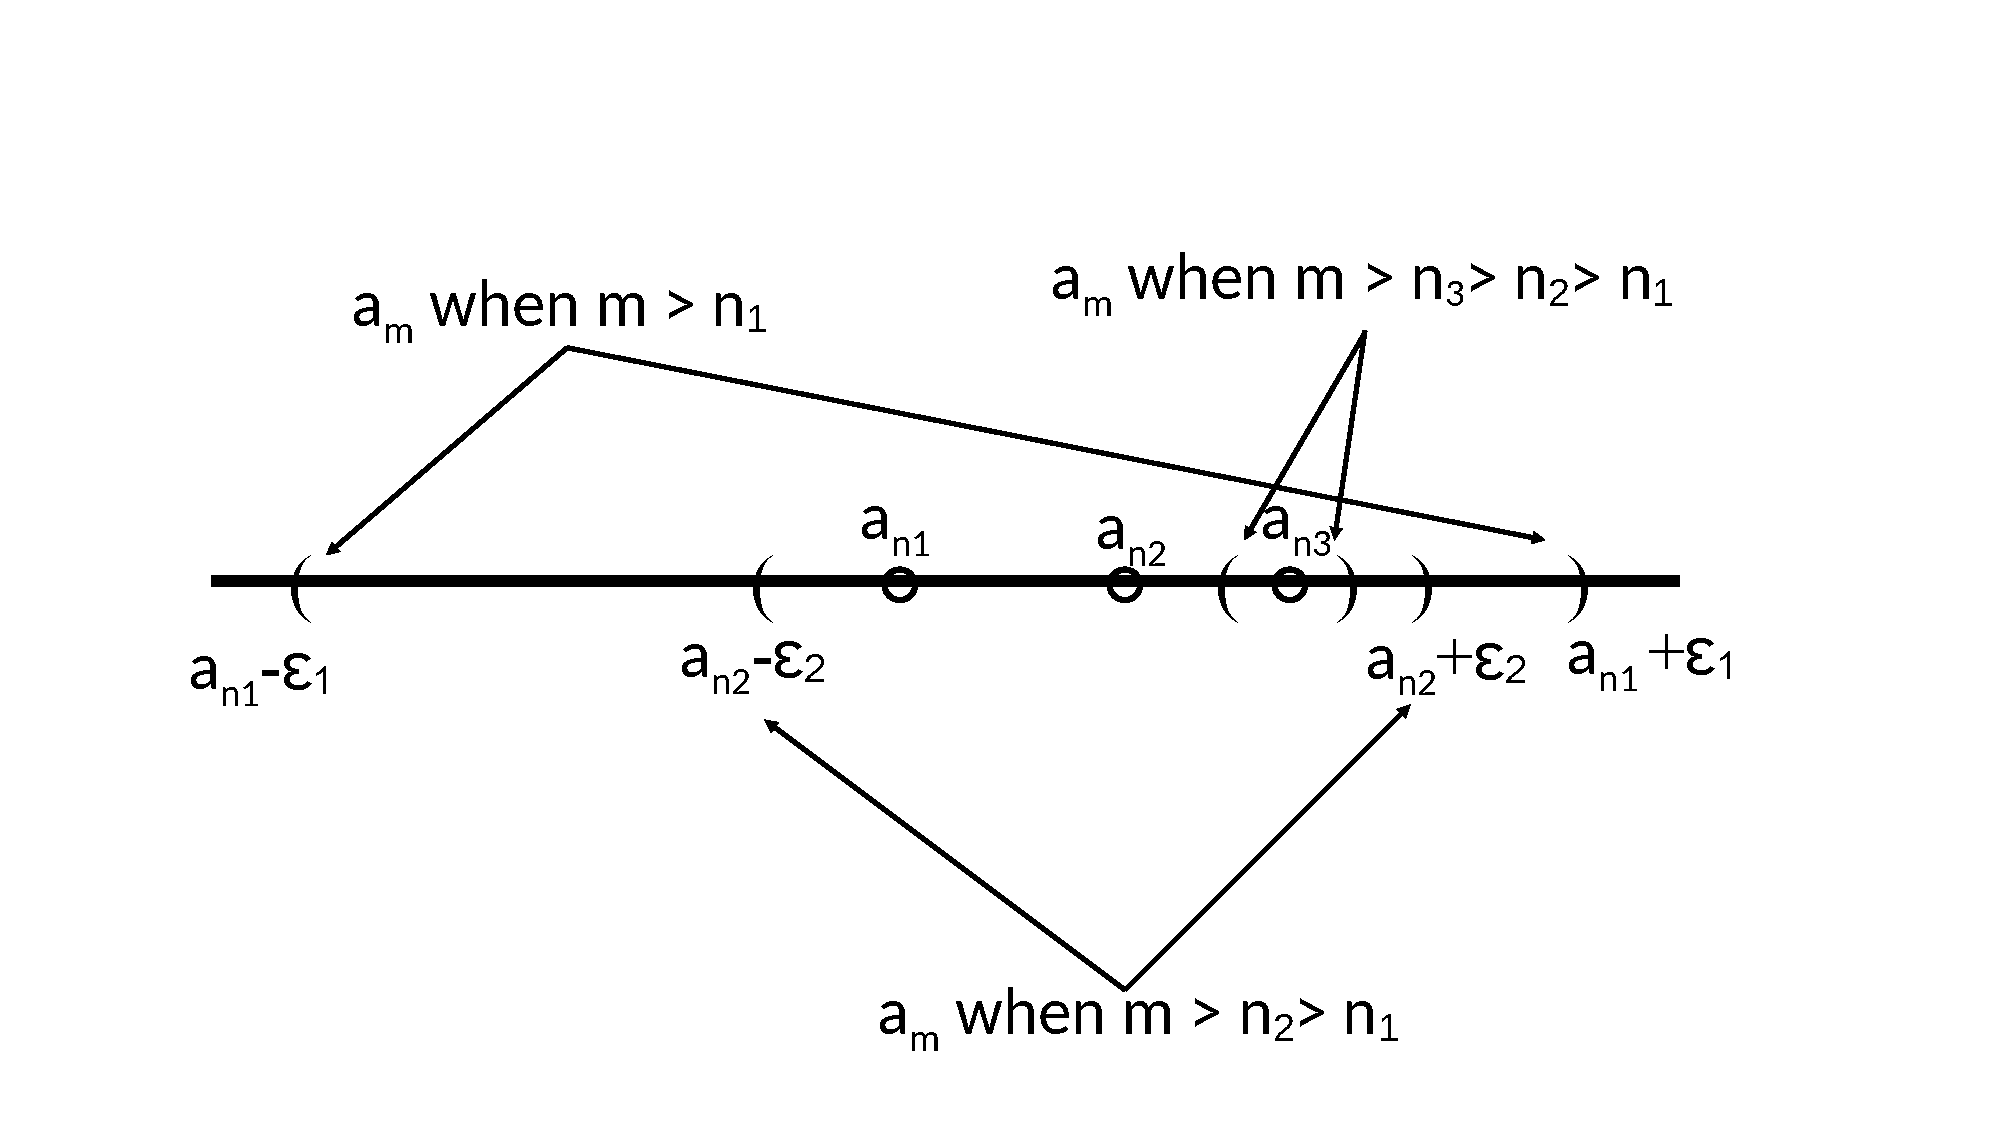
\includegraphics[scale=0.25]{cauchy}
\end{center}
\caption{Convergence of a Cauchy Sequence \label{fig:cauchy}}
\end{figure}

\subsubsection{Exercises}
\begin{itemize}
\item Suppose $f$ is allowed to be non-continuous at just one point in $[a,b]$; can we still guarantee the existence of $a < x' < b$ such that $f(x') = y'$?
\item Prove that every convergent sequence is a Cauchy sequence; this is true with or without our assumption.
\item Prove that every decimal expansion converges -- i.e., as promised, every infinite series of the form
\begin{equation}\label{eq:decimalExpansionExercise}
\sum \frac{d_n}{10^n}
\end{equation}
 (where each $d_n$ is a digit, i.e. an integer in the range 0 to 9) converges.
\item Let $\lim a_n = \alpha$. Prove that $\alpha$ can be represented by a decimal expansion -- i.e. there is a series of the above form which converges to $\alpha$.
\end{itemize}


\subsection{The Intermediate Value Theorem}
We now prove that the convergence of Cauchy sequences -- i.e. the completeness of the real numbers --``fills up" the number line enough to yield the intermediate value property. Let $a,b,f,y'$ be as in claim (\ref{claim:intermediateValue}). Given the tools at our disposal, there is only one thing to try to do: find a Cauchy sequence $\{x_i\}$ such that $\lim f(x_i) = y'$. Then completeness means that $\{x_i\}$ converges to a real number $x'$, and continuity implies $f(x')=y'$.

Geometric intuition tells us that that somewhere the graph of $f$ must cross over the horizontal line $y=y'$, so our strategy is to narrow down where this happens.  We begin by dividing the problem in half, letting $x_0=a, x_1=b$ and $x_2 = \frac{a+b}{2}$. There is nothing more to prove if $f(x_2)=y'$, otherwise we continue with
\[
x_3 = 
\begin{cases}
a+\frac{b-a}{4}, &\text{if $f(x_2)<y'$}\\
a+3\frac{b-a}{4}, &\text{if $f(x_2)>y'$}\\
\end{cases}
\]
i.e we go halfway toward one endpoint or the other, in whatever direction will put the crossover point between $x_2$ and $x_3$. We continue in this manner (see figure \ref{fig:IVP}); after selecting $x_j$ we limit our attention to an interval of width $\frac{b-a}{2^j}$, which is either $(x_i,x_j)$ with $f(x_i) < y < f(x_j)$ or $(x_j,x_i)$ with $f(x_j) < y < f(x_i)$ (for some $i<j$); then $x_{j+1}$ will be the midpoint of this interval.

We can stop if we ever get $f(x_j)=y'$: otherwise the $\{x_i\}$ are a Cauchy sequence, because the tail $x_j, x_{j+i} \cdots$ is contained within an interval of width $\frac{b-a}{2^j}$. We claim its limit is the required $x'$. Consider two subsequences of $\{x_i\}$: one consisting of all $x_k$ with $f(x_k) < y'$, call this sequence $\{x^{-}_i\}$, and the other terms  $\{x^{+}_i\}$. If both of these subsequences are infinite, they both converge to $x'$. Now the sequence $f(x^{-}_i)$ has all terms less than $y'$, so its limit, which is $f(x')$, must be less than or equal to $y'$; similarly $f(x')=\lim f(x^{+}_i) \geq y'$, so $f(x')=y$.

\begin{figure}
\begin{center}
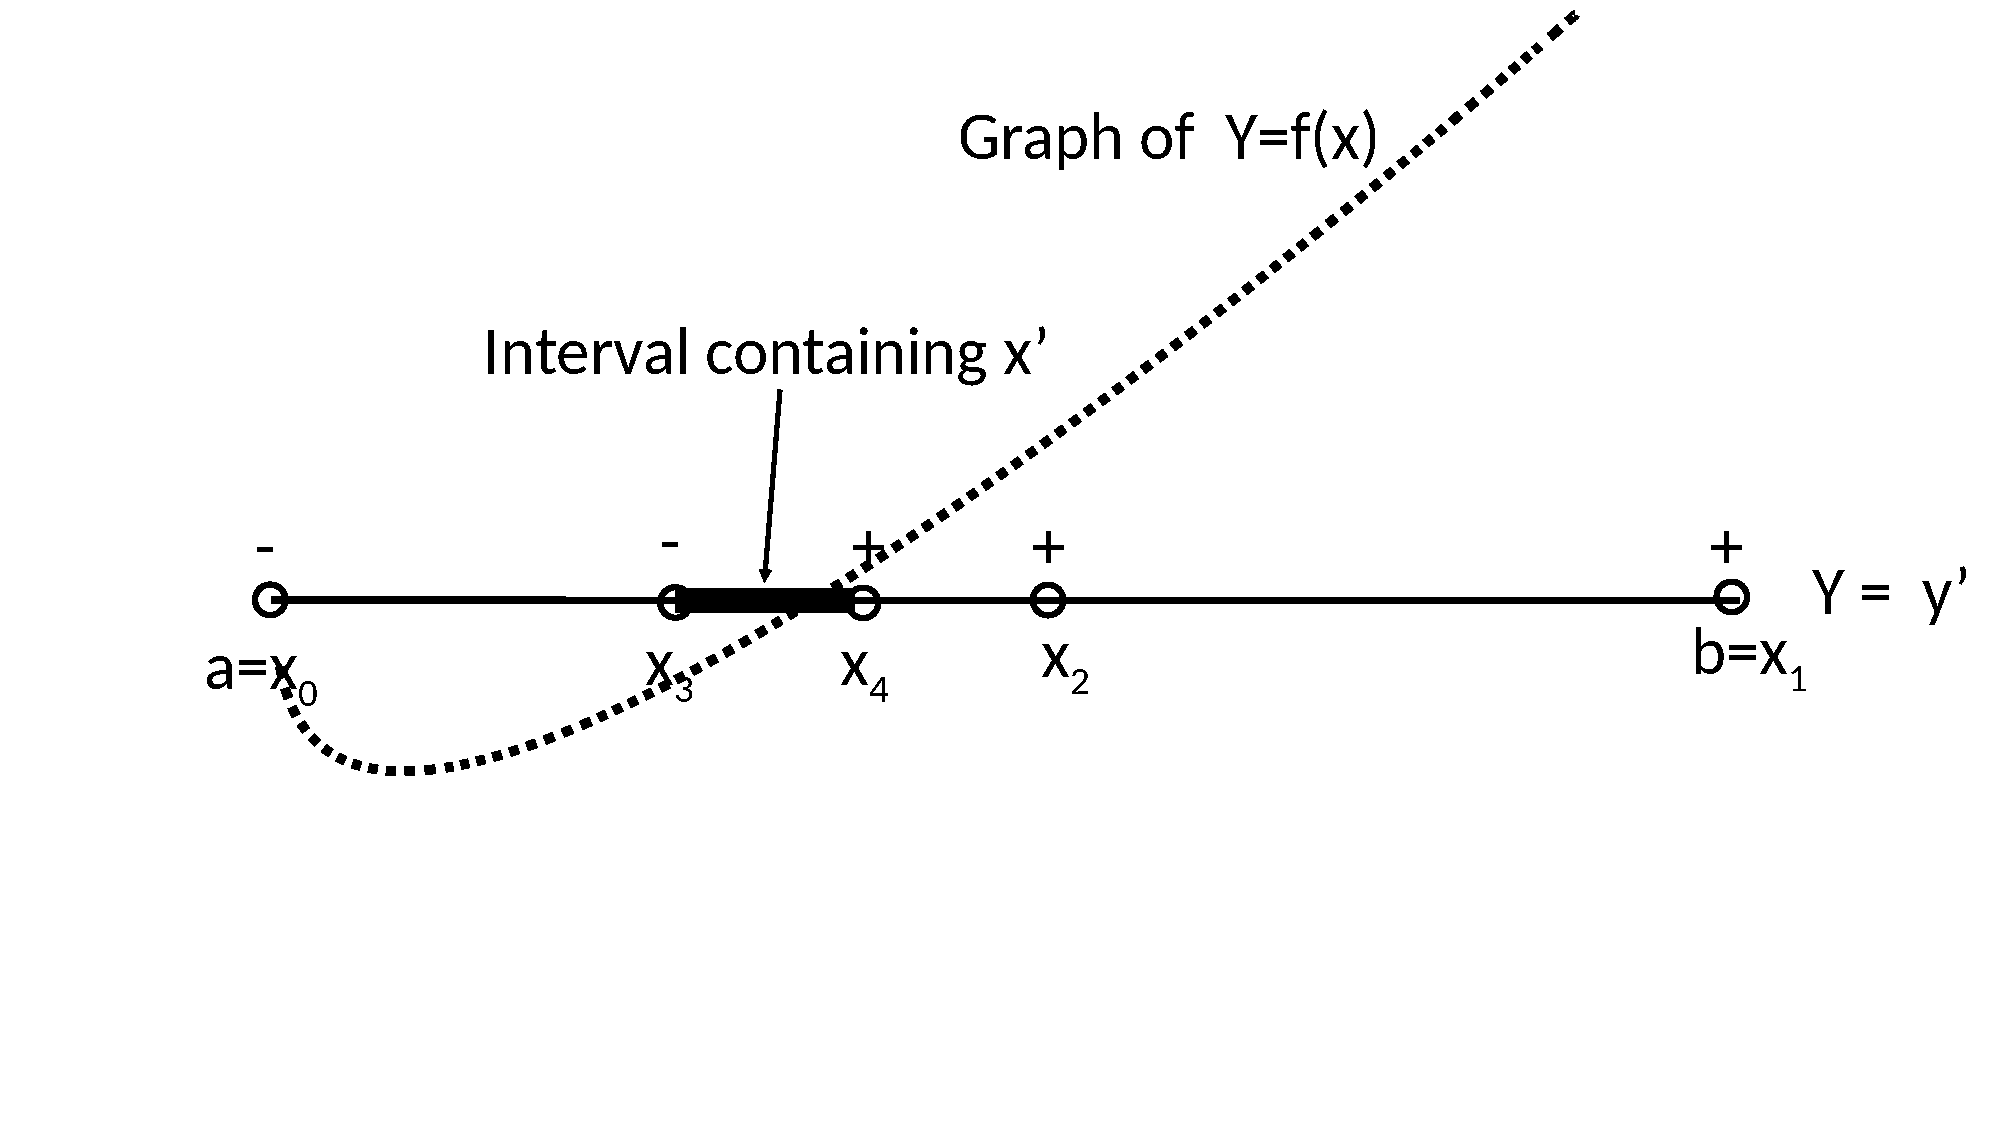
\includegraphics[scale=0.25]{IVP}
\end{center}
\caption{Proof of the Intermediate Value Property \label{fig:IVP}}
\end{figure}


Finally we must dispense with the possibility that one of these subsequences, say $\{x^{+}_i\}$, is finite. In that case there must be a largest index $M$ at which $f(x_M)>y'$. From the definition of the sequence we would necessarily have $x_i = M - \frac{b-a}{2^i}$ for every $i>M$. But that is impossible: we would get $x' = \lim x_i = x_M$ and thus $\lim f(x_i) = f(x_M) > y'$ while every $f(x_i) < y'$.

%It is a useful definition because it captures what makes a sequence convergent without making any explicit reference to the limit; if we deny the existence of irrationals it makes no difference, a Cauchy sequence is still a Cauchy sequence.

{\color{red}
\subsubsection{Exercises}
Least upper bounds; maximum/minimum  of continuous function on a closed interval.
%Need intermediate value for chain rule? inverse functions?
}

\subsection{Behavior of Continuous Functions}\label{sec:behaviorOfContFuncs}
This section is optional, i.e. subsequent material does not depend on it. Since it is optional we will cheat a bit and make use of the sine function even though we have not formally defined it. We know that its graph crosses the $x$-axis infinitely often, at each $x_0=k\pi$. Thus the graph of $f(x) = \sin(1/x)$ looks like figure ??; in any open interval around zero it changes direction and crosses the $x$-axis infinitely many times. It will be discontinuous at zero no matter what value we assign to $f(0)$; different sequences $a_n$ with $\lim a_n = 0$ could have $\lim f(a_n)$ equal to any $-1 \leq \alpha \leq 1$, or the limit might not exist (exercise: give examples of such). But we can tame this wildness somewhat by defining
\[
g(x) = \begin{cases}
|x|\sin(1/x), &x \neq 0\\
0, &x = 0
\end{cases}
\]
to get something that looks like figure ??. Now the infinite fluctuations keep getting smaller, and $\lim a_n = 0$ does imply $\lim f(a_n) = 0$ because $|f(a_n)| \leq |a_n|$ (exercise: finish the proof). Thus $g$ is continuous everywhere. Yet we still cannot imagine drawing the entire graph, and we doubt that any object could move this way, as it would require infinitely many changes of direction in a finite space and time.

\subsubsection{Exercises}
Anything else?

%\subsection{Limit of a function at a point}
%Whether or not a function $f$ is continuous at $\alpha$, we define
%
%\begin{defn}
%Let $f$ be defined at all points on an open interval $I$ containing $\alpha$, except perhaps $\alpha$ itself. If there is a $\beta$ such that
%\[\lim f(a_n) = \beta\]
%for all convergent sequences $a_n$ with values in $I\setminus\{\alpha\}$\footnote{This is the notation for the \emph{difference} of two sets: $A \setminus B$ consists of all elements of $A$ that are not in $B$. Here it says we remove the single point $\alpha$ from $I$.}
%and $\lim a_n = \alpha$, we write
%\[\lim_{x \to \alpha} f(x) = \beta\]
%and call $\beta$ the limit of $f$ at $\alpha$.
%\end{defn}
%
%We can apply this definition to something like
%\[
%g(x) = \begin{cases}
%1, &x \neq 0\\
%0, &x = 0
%\end{cases}
%\]
%which is discontinuous at zero but has $\lim_{x\to0} g(x) = 1$; note that it is essential in the definition to exclude $\alpha$, so that we do not consider the limit of $g(a_n)$ where $a_n=0$ for all $n$.
%
%Similarly let $f(x) = \frac{x^2-1}{x-1}$; since $x^2-1 = (x-1)(x+1)$, this function is equal to $x+1$ except for being undefined at 1. So it cannot be continuous at 1, but we have $\lim_{x\to1}f(x) = 2$.
%
%Now at this point one might fairly ask, ``why bother"? The function $g$ looks somewhat ridiculous, and why would we ever write $\frac{x^2-1}{x-1}$ when we could just write $x+1$? We will see in a later chapter how such things might arise, but a good motivating example is
%\[
%h(x) = \frac{\sin(x)}{x}\ .
%\]
%The graph looks like figure ??; if you do not believe it, just try calculating $h(0.01), h(0.001)$ et cetera; it looks like $\lim_{x\to0} h(x)=1$. But there is no immediately apparent way to cancel out the $x$ to get an expression that can be evaluated at zero.
%
%Our definitions immediately give us
%\begin{thm}
%A function $f$ is continuous at $\alpha$ if and only if 
%\[\lim_{x\to\alpha}f(x)=f(\alpha)\]
%\end{thm}
%


\pagebreak
\section{Derivatives}
On 20 July 1969 the Apollo 11 lunar module landed on the moon, 112.75 hours after being launched. Since the distance from Earth to the moon is always at least 362,600 km, the average speed of the trip must have been at least 3216 km per hour. The astronauts would not have had a good time hitting the lunar surface at that speed, but of course they did not; they touched down gently at about one km per hour. What matters for a soft landing is vertical speed \emph{at the moment of touchdown}; but what does that mean? This moment lasts zero seconds, during which the ship travels zero kilometers, and an average speed of ``zero divided by zero" does not make much sense. The idea of speed at one moment in time -- better known as \emph{instantaneous velocity} -- can be defined using limits.\footnote{In fact this problem was one of the things that first led mathematicians to come up with the whole idea.}

We encountered a problem trying to compute the average velocity of the lunar module at the moment when it touches the moon, and we did not get anything useful by considering its average velocity over the entire Earth-moon voyage, but there is no difficulty in considering its average velocity over the last, say, second before touchdown, which should be more relevant to the softness of the landing. And we can continue in this manner, taking the average velocity in the last half second, quarter second and so on; this gives us a sequence of velocities which  should give increasingly accurate descriptions of what is happening precisely at touchdown, so we will define the instantaneous velocity to be the limit of this sequence.

Velocity is the rate of change of an object's position, but the same idea applies to the rate of change of any quantity over time; our changing quantity will be the value of some function $f(x)$, which changes as $x$ changes. The average rate of change of $f(x)$ in the interval $a \leq x \leq b$ is
\[
\frac{f(b)-f(a)}{b-a}
\]
In particular if $f(x)$ is the location of a moving object at time $x$, this becomes the familiar ``distance divided by time". Our idea was to keep making the interval $b-a$ smaller, shrinking toward zero without ever quite getting there. Above we suggested intervals of lengths $1, 1/2, 1/4 \cdots$ but everything should work out the same if we consider $0.1, 0.01, 0.001 \cdots$, or even if we stagger toward zero in some less regular-looking way. 

When considering an abstract function (i.e. ``just numbers" with no measurement units), instantaneous velocity is called the \emph{derivative} of the function. Thus we arrive at:
\begin{defn}\label{def:derivative}
Let $f$ be continuous at $a$. The \emph{derivative} of $f$ at $a$, written $f'(a)$, is
\[
\lim \frac{f(a+\delta_n) - f(a)}{\delta_n}. 
\]
if this limit exists, is finite, and is the same for all sequences $\delta_n$ such that $\lim \delta_n = 0$ and for all $n$ $\delta_n \neq 0$.
\end{defn}
A function that has a derivative at $a$ is said to be \emph{differentiable} at $a$.

As we did when we first introduced limits, we will, to get started, not give much thought to how the supposed limit might fail to exist; we will soon see that for most ``normal-looking" functions, it does exist. We do note one 
subtle difference between this definition and the touchdown example: in computing $f'(a)$ we do not just consider ``times before $a$" (i.e. $x<a$), but also times after -- i.e. each $\delta_n$ could be positive or negative (since the limit is zero we can have a mix of both). 

\subsection{Tangent Lines}
{\color{red}Slopes, constant rate of change.}

\subsection{Polynomials}
Proof that derivative of $x^2$ is $2x$:
\[
\lim \frac{(x+d_n)^2 - x^2}{d_n} = \lim\frac{2xd_n + d_n^2}{d_n} = \lim 2x + \lim d_n = 2x + 0 = 2x
\]
These equalities are valid for any $d_n$ approaching zero.

%Are fractional exponents equally easy? Can apply inverse theorem to $r^\mbox{th}$ root, but note that square root also comes right out of product rule.


\subsection{Differentiation Formulae}
Sum $f+g$ is almost immediate.

We now consider differentiation of products:
Let $h(x) = f(x)g(x)$ with $f$ and $g$ differentiable. Direct application of the definition gives $h'(x)$ as
\[
\lim \frac{f(x+\delta_n)g(x+\delta_n)-f(x)g(x)}{\delta_n}
\]
if this limit exists. What can we do here? We would like to hope that $h'(x)$ can somehow be expressed as some combination of $f'(x)$ and $g'(x)$, but how could we extract such things from what we have? Since $\delta_n$ is approaching zero, note that we have something that looks very close to $f(x)g'(x)$; if only we could replace $f(x+\delta_n)$ with the barely different $f(x)$ we could pull out $f(x)$. So we will write $f(x+\delta_n)$ as $f(x)+ Z$ and see what we can do with $Z$. Of course the ``error term" $Z$ is just  $f(x+\delta_n) - f(x)$, and we get
\[
\lim \frac{[f(x)+f(x+\delta_n) - f(x)]g(x+\delta_n)-f(x)g(x)}{\delta_n}
\]
which is
\[
\lim \frac{f(x)g(x+\delta_n)-f(x)g(x)}{\delta_n} + \frac{[f(x+\delta_n) - f(x)]g(x+\delta_n)}{\delta_n}
\]
thus
\[
f(x)g'(x) + \lim g(x+\delta_n) \lim \frac{[f(x+\delta_n) - f(x)]}{\delta_n}
\]
By continuity, we have $\lim g(x+\delta_n) = g(x)$ and thus

\begin{thm}[Product Rule]\label{thm:productRule}
Let $h(x)=f(x)g(x)$; if $f$ and $g$ are differentiable at $x$ then so is $h$ and
\[
h'(x) = f(x)g'(x) + f'(x)g(x)
\]
\end{thm}

Note that this is symmetrical in $f$ and $g$, as it must be since $f(x)g(x)=g(x)f(x)$. 

Next we consider \emph{composition} of functions, i.e. functions of the form $h(x) = f(g(x))$. If we can handle composition, we can handle just about any formula we can write: in later chapters we will see how to take the derivative of functions like $\log(x)$ and $\sin(x)$ and $2^x$, and then composition takes us to expressions like
\[
2^{\cos(\sqrt{\sin(\log x))}}
\]

But we are getting ahead of ourselves. The derivative of $h(x) = f(g(x))$ is by definition
\begin{equation}
\label{eq:chainRule1}
\lim \frac{f(g(x+\delta_n)) - f(g(x))}{\delta_n}
\end{equation}
We might be forgiven if our first response to the question of what to do with this beast is along the lines of ``!?!?!", but let's take a deep breath and see what we have. As before, we hope that we can express this as some conglomeration of $f'(x)$ and $g'(x)$. Remember that the derivative of $f(x)$ involves evaluating $f$ at two very close points, and that is exactly what we have in our numerator; the close points are $g(x)$ and $g(x+\delta_n)$. The difference between these, i.e. $\delta'_n = g(x+\delta_n)-g(x)$, gives us a sequence that approaches zero (because we have assumed $g$ continuous): by definition this sequence $\delta'_n$ must work just fine for finding the derivative. Note however that we are taking the derivative of $f$ at $g(x)$ instead of at $x$. To get something that looks like $f'(g(x))$ we  need to have division by $g(x+\delta_n)-g(x)$, but that problem is easily fixed: we can  we rewrite (\ref{eq:chainRule1}) as

\[\label{eq:chainRule2}
\lim \frac{f(g(x+\delta_n)) - f(g(x))}{g(x+\delta_n)-g(x)} \frac{g(x+\delta_n)-g(x)}{\delta_n}
\]
Now the part on the left is indeed $f'(g(x))$, and the rest is precisely the definition of $g'(x)$, thus
\begin{thm}
The derivative of $f(g(x))$ is
\[
f'(g(x))g'(x)
\]
if $g$ is differentiable at $x$ and $f$ is differentiable at $g(x)$.
\end{thm}
This result is called the ``chain rule".
{\color{red} NOTE: this proof needs more care since we could have division by zero!

Show that chain rule gives consistent result for $x^n$; can derive $nx^{n-1}$ from product or composition or directly.}

%Hard to give nice chain-rule examples without trig/log/exp functions, but can show consistency among various ways to write algebraics. Spivak actually just states the trig derivatives as known facts for the sake of examples; we can just introduce ``arbitrary" functions $S(x)$ and solve problems in terms of $S'(x)$; find the derivative of $S(x + S(x))$ et cetera.

%We have cheated a bit in the chain rule; in defining the derivative we really need to enforce $\delta_n \neq 0$, so be careful. Indeed might make more sense to restrict to monotonic, but then need to demonstrate existence of monotonic sequence.



\subsection{Exercises}
\begin{itemize}
\item Find the derivative of $f(g(h(x)))$ (assume all three functions are defined and differentiable everywhere -- or even better, state explicitly what we must assume for this derivative to make sense)
\item Find a function $f$ such that $f'(x) = 2x^3+1$. Is there more than one such function?
\end{itemize}


\subsection{Tangent Lines, Again}
We noted earlier that the derivative is the slope of the tangent line, and that the graph of $f(x)$ looks a lot like the tangent line if we stay close to $x_0$. Every calculus text emphasizes this, but most do not point out that the geometrical intuition can be expressed in a precise algebraic way. For that we need another definition:
\begin{defn}
A function $\nu$, continuous at $x_0$, is \emph{negligible} at $x_0$ if
\[
\lim \frac{\nu(x_0 + \delta_n)}{\delta_n} = 0
\]
For any sequence such that $\lim \delta_n = 0$
\end{defn}
Henceforth we usually leave the ``at $x_0$" implicit. Note being negligible implies, and is stronger than, merely asserting $\nu(x_0+\delta_n)$ goes to zero; the idea is that $\nu(x_0+\delta_n)$ approaches zero \emph{faster} than $\delta_n$ does. The difference between $f$ and its tangent-line approximation is a negligible function, i.e.
\begin{thm}\label{thm:linearApprox}
Let $f$ be differentiable at $x_0$. Then
\[
f(x) = f(x_0) + f'(x_0)(x-x_0) + \nu(x)
\]
for some function $\nu(x)$ which is negligible at $x_0$.
\end{thm}
\begin{proof}
{\color{red} pretty straightforward from definitions}
\end{proof}

This view of the derivative gives us a different way to prove some theorems. Let's take another look at the product rule (theorem \ref{thm:productRule}); can we write $f(x)g(x)$ in a form that looks like theorem \ref{thm:linearApprox}? We now know that
\[
f(x)g(x) = \{f(x_0) + f'(x_0)(x-x_0) + \nu_f(x)\}\{g(x_0) + g'(x_0)(x-x_0) + \nu_g(x)\}
\]
where $\nu_f, \nu_g$ are both negligible. It looks like we will get quite a mess here, multiplying a pair of 3-term expressions to get a 9-term expression. But this is definitely a time to work smarter, not harder. All our previous results about limits and continuous functions tell us that:
\begin{itemize}
\item the sum of two negligible functions (at the same $x_0$) is negligible
\item $\nu(x)h(x)$ is negligible if $h$ is continuous at $x_0$
\end{itemize}
Therefore \emph{all} of the terms involving $\nu_f$ or $\nu_g$ are negligible and can be combined into a single $\nu(x)$; what we are left with is
\begin{flalign*}
f(x)g(x) &= \\
   &f(x_0)g(x_0) + (f(x_0)g'(x_0)+f'(x_0)g(x_0))(x-x_0) \\
   &+ f'(x_0)g'(x_0)(x-x_0)^2+ \nu(x)
\end{flalign*}
and our previously-derived formula from the product rule has just appeared in the middle of things. We finish up by noting that $f'(x_0)g'(x_0)(x-x_0)^2$ is negligible (exercise below) and can be absorbed into $\nu(x)$.

To really make this a proof of the product rule, we need the converse of theorem \ref{thm:linearApprox}, which asserts that, if $\nu$ is negligible, the constant being multiplied by $(x-x_0)$ cannot be anything but the derivative at $x_0$: that is left as an exercise. It might look at first glance like we have only demonstrated something about the derivative at a single point, but since $x_0$ could equally well be any point at which $fg$ is differentiable we are done.

We need one more theorem to fill out our toolbox of differentiation formulae:

\begin{thm}\label{thm:multInverseDeriv}
If $f$ is differentiable at $x_0$ and $f(x_0) \neq 0$ then the derivative of $1/f(x)$ is
\[
\frac{-f'(x)}{f(x)^2}
\]
\end{thm}
\begin{proof}
Having introduced theorem \ref{thm:linearApprox}, we might as well use it at least one more time, so we begin with
\[
\frac{1}{f(x)} = \frac{1}{f(x_0) + f'(x_0)(x-x_0) + \nu(x)}
\]
This is not quite as nice as the product rule since we do not have $1/f(x_0)$ by itself, but we can make it appear with the right algebraic manipulation. In general
\[
\frac{1}{A + a} = \frac{1}{A} - \frac{a}{A(A+a)}
\]
so in particular
\[
\frac{1}{f(x)} = \frac{1}{f(x_0)} + \frac{-f'(x_0)(x-x_0)-\nu(x)}{f(x_0)(f(x_0)+f'(x_0)(x-x_0)+\nu(x))}
\]
as with the proof of the product rule, we can simplify this quite a bit by rolling up expressions that we know are negligible; in this case, $\nu(x)$ divided by something that we know is \emph{not} zero at $x=x_0$:
\[
\frac{1}{f(x)} = \frac{1}{f(x_0)}
+ \frac{-f'(x_0)}{f(x_0)^2+f(x_0)f'(x_0)(x-x_0)+\nu_0(x)}(x-x_0) - 
  \nu_1(x)
\]
This is getting close to our claimed result; another application of rewriting $\frac{1}{A+a}$ is needed to clean up the denominator of the fraction, pulling out another negligible term to obtain
\[
\frac{1}{f(x)} = \frac{1}{f(x_0)}
+ \frac{-f'(x_0)}{f(x_0)^2}(x-x_0) - \nu_2(x)
\]
\end{proof}


\subsubsection{Exercises}
\begin{itemize}
\item Derive a general formula for the derivative of $x^{-n}$ and $x^{-n/m}$.
\item Find the derivative of $\frac{f(x)}{g(x)}$
\item Prove that $f'(x_0)$ is the \emph{only} real number $\mu$ such that $f(x) = f(x_0) + \mu(x-x_0) + \nu(x)$ with $\nu(x)$ negligible, and that any function of this form is differentiable at $x_0$. Note this means we could just as well have \emph{defined}  $f'(x_0)$ as this unique $\mu$.
\item Prove theorem \ref{thm:multInverseDeriv} directly from definition \ref{def:derivative}.
\item Prove the claim made above that $f'(x_0)g'(x_0)(x-x_0)^2$ is negligible.
\end{itemize}
%this might be more distracting than helpful; material on closest linear approximation is essentially a better version of this idea
%\subsection{Some Interpretations}
%
%Chain rule has a nice intuitive interpretation. $f'(g(x))$ tells us how fast $f(t)$ is changing as $t$ moves toward the number $g(x)$ ``at a steady rate"; note that $g(x)$ is just a number, it does not matter that we can write this number using the function $g$. The factor $g'(x)$ tells us how much $f(t)$ is slowed down or sped up if $t$ is driven by $g$; i.e. $t=g(t')$ where now $t'$ is time moving toward $x$ at a steady rate. 
%
%Rectangle interpretation of product rule.
%
%
%Can tangent line to circle be expressed in terms of trigonometric functions?


\subsection{Increasing and Decreasing Functions}
{\color{red}
Might start a new chapter here. 

Positive rate of change means increasing.

%{changed our mind on this one} This is where we introduce and motivate the supremum property. In exercise, note that Archimedean property is a consequence.

Consider max point of function. The derivative should not be positive, that would mean we could get a larger value by moving a bit to the right. Similarly cannot be negative.

Max/min at zero derivative; Increasing implies nonnegative derivative.
}%end \color{red}

\subsection{Second Derivative}
{\color{red}Convexity and Concavity}


\subsection{Non-Differentiable Functions}
{\color{red}Absolute value is example of non-differentiability; sequences approaching zero from the left and from the right give different results.} %another case where sequence-based approach simplifies

If $\delta_n = 1/n$ then
\[
\lim \frac{|\delta_n| - |0|}{\delta_n} = \frac{\delta_n}{\delta_n} = 1
\]
but if $\delta_n = -1/n$ then
\[
\lim\frac{|\delta_n| - |0|}{\delta_n} = \frac{-\delta_n}{\delta_n} = -1
\]
The point here is that $|x|$ looks like $x$ on one side of the origin and like $-x$ on the other side; we can get endless examples of continuous non-differentiable functions by ``gluing together" two unrelated differentiable functions that happen to satisfy $f(x_0)=g(x_0)$ at some $x_0$ (figure ??).


\subsubsection{Exercises}
%Path of a point on a wheel is also non-differentiable where point touches ground.
\begin{itemize}
\item In the definition of the derivative, the assumption of continuity is essential; show that the required limit cannot exist if $f$ is not continuous.
%(true since definition requires numerator to be approaching zero). If derivative is $\alpha$ then when $|\delta_n| < \varepsilon$
%\[
% (\alpha - \varepsilon)\varepsilon \leq f(x + \delta_n) -f(x) \leq (\alpha + \varepsilon)\varepsilon
%\]
\item If $f'(x)=0$ for all $x$, then $f$ is a constant function.
\end{itemize}

%Compute derivative of area under a curve as prelude to integration -- how much of that can be turned into an exercise? But derivative of $f$ when $f$ itself is unknown might be overly abstract -- as always, want to present with proper motivation.

\pagebreak
\section{Trigonometric Functions}
We assume that the reader is already familiar with sines and cosines and will not repeat the well-known definitions here. But before we can do calculus with these things, we have to consider a mildly subtle point about what units we should  use to measure angles. When computing distance or speed, the absolute sizes of our units do not really matter; the meter and the foot are just conventions, we can just as well take one unit of length to be the distance from earth to the sun or the diameter of an atom. But trig functions are a bit different. A right angle is a right angle, and we cannot do anything without knowing how many units make a right angle. Traditionally we say ninety, because that makes a lot of computations come out cleanly -- a half, third, fifth, or sixth of a right angle is a whole number of degrees.\footnote{This was a big deal back in the days when all computations had to be done by hand! Also the sun moves a quarter of the the way around the zodiac in about 90 days -- i.e. roughly one degree per day, which was useful for astronomy.}

But there is another, equally standard approach, which works far better for our purposes. We will imagine all angles drawn at the center of a circle of radius ``one unit", and the measure of an angle is the length of the arc it spans. Since the circumference of our circle is $2\pi$, a right angle is one-quarter of the circumference, or $\pi/2$.  Since $r=1$, the area of our circle is $\pi$, and we can just as well say that an angle is measured as double the area of its wedge. This is known as measuring angles in \emph{radians}. From here forward, ``degrees" are banished to the dustbin of history! When measuring angles in radians, it can be useful to imagine walking counter-clockwise around a unit circle, starting at $(1,0)$; if we have gone distance $\theta$ along the arc, then we are at the point $(\cos(\theta), \sin(\theta))$. If $\theta < 0$, we are moving clockwise.
%add diagram for angle measurement

If we are going to combine calculus with trigonometry, our first order of business is to find the derivatives of trig functions. The derivative of $\sin(x)$ is
\[
\lim \frac{\sin(x+d_n)-\sin(x)}{d_n}
\]
Where $\lim d_n = 0$. What can we do with such an expression? It looks like the summation rule for sines is the thing to try here; we recall from high-school trigonometry that
\[
\sin(\alpha + \beta) = \sin(\alpha)\cos(\beta) + \sin(\beta)\cos(\alpha)
\]
Ideally we should prove this formula, but since it is so well-known we will give ourselves a bit of a break and just take it for granted. Applying  it to our problem yields
\[
\sin'(x) = \lim \frac{\sin(x)\cos(d_n) + \sin(d_n)\cos(x)-\sin(x)}{d_n}
\]
Believe it or not, this is progress! The factors $\sin(x)$ and $\cos(x)$ are constants which we can pull out of the limit if we break up the sum.  We get
\[
\sin'(x) = \sin(x)\lim \frac{\cos(d_n) - 1}{d_n} + \cos(x)\lim \frac{\sin(d_n)}{d_n}
\]
How would we evaluate such limits? We do not have a ``formula" for sines and cosines, which means we cannot get very far by algebraic manipulation alone; we need to reason about the geometric meaning of our equation. So we draw a diagram as in figure \ref{fig:sine}.

Taking one thing at a time, we will first attack $\lim \sin(d_n)/d_n$. The shaded area in the diagram is $d_n/2$. We will associate an angle with the area of a wedge (rather than with the length of an arc) because it is much easier to reason about areas: if one figure is completely inside another, we know that the interior figure has smaller area, even if we know nothing else about what these areas are. This suggests using our results about limits and inequalities; we will trap our challenging limit between two things we can calculate more easily.

We thus want to find the largest simple shape contained in the wedge, and the smallest simple shape that contains the wedge, where ``simple" means something whose area we know how to compute. In the diagram, we can see that there is a right triangle entirely inside the wedge; if we add the box to the right, we have a trapezoid which contains the wedge. Thus
\[
\frac{1}{2}\sin(d_n)\cos(d_n) < d_n/2 <  \frac{1}{2}\sin(d_n)\cos(d_n) + \sin(d_n)\left(1 - \cos(d_n)\right)
\]
A little algebraic simplification takes us to
\[
\sin(d_n)\cos(d_n) < d_n <   \sin(d_n)\left(2 - \cos(d_n)\right)
\]

\begin{figure}
\begin{center}
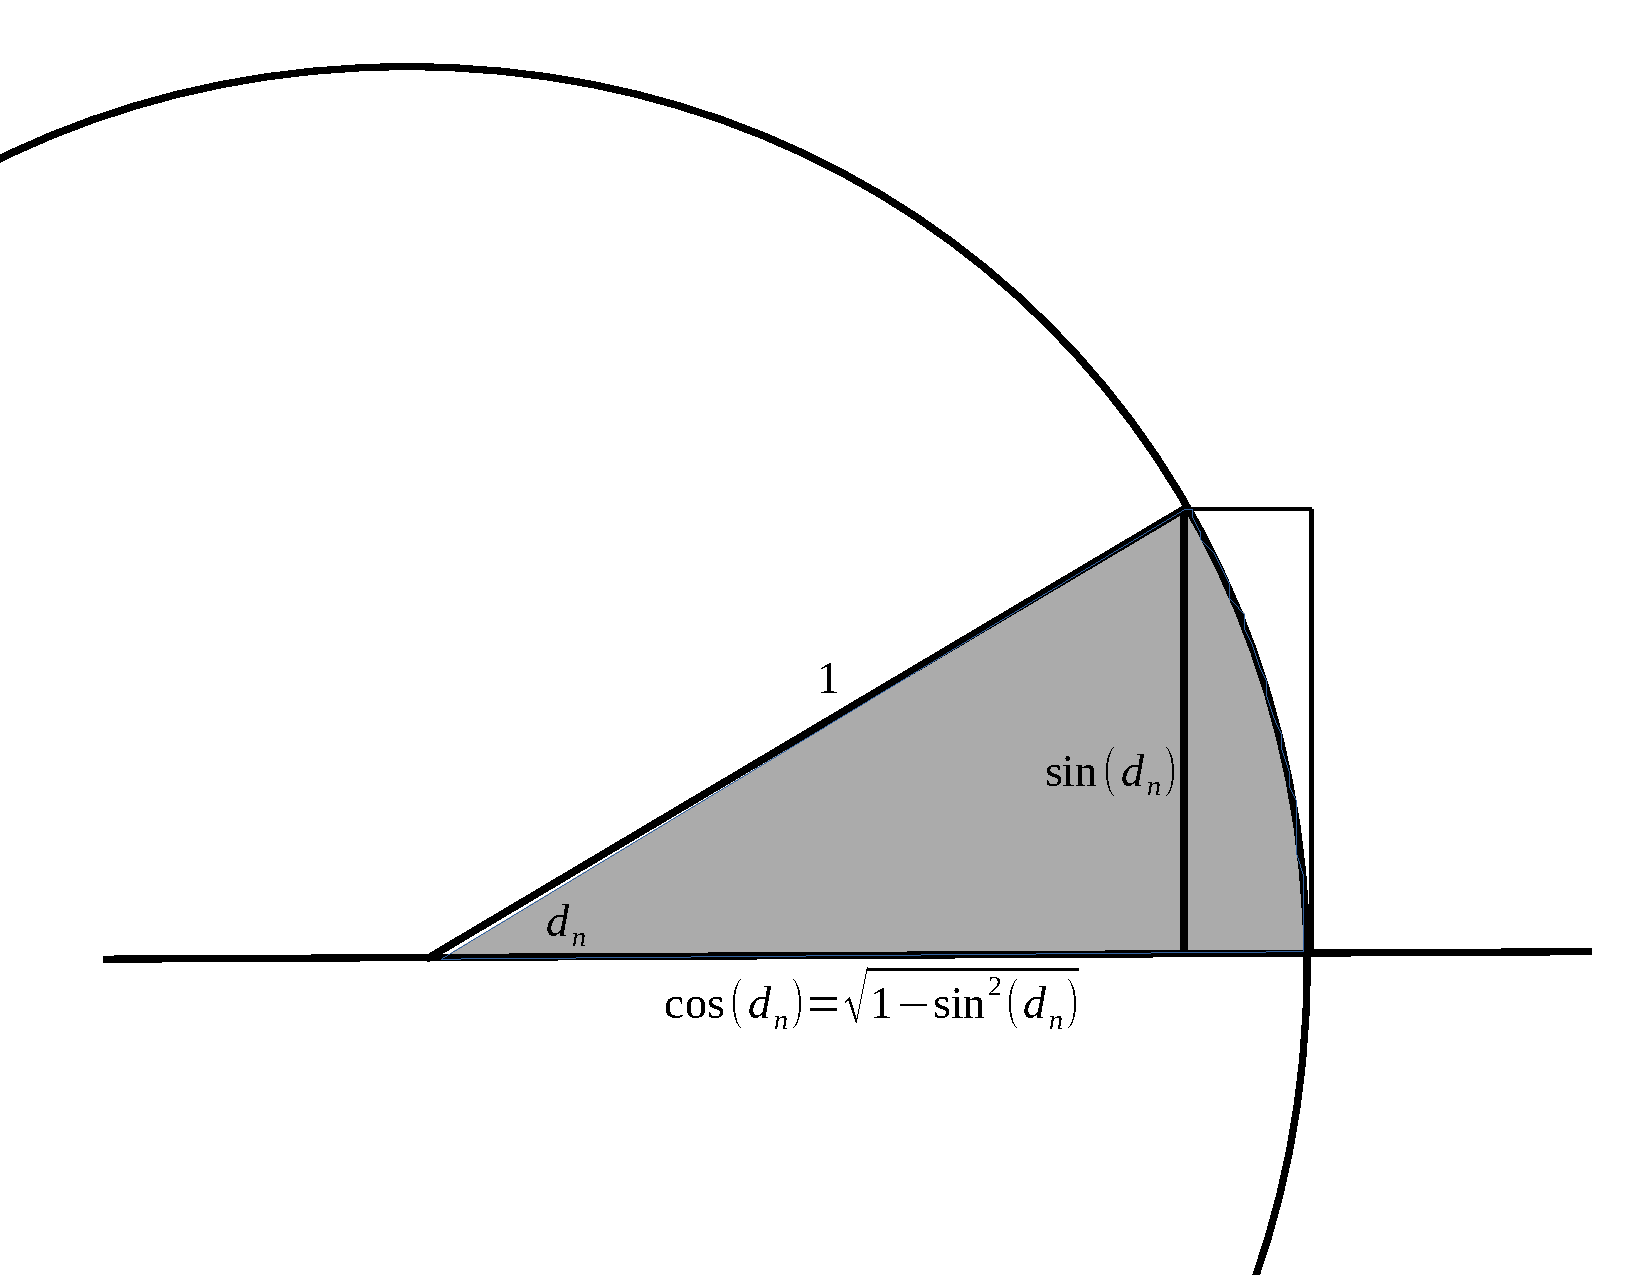
\includegraphics[scale=0.33]{trig}
\end{center}
\caption{Derivative of $\sin(x)$\label{fig:sine}}
\end{figure}


Dividing $\sin(d_n)$ into each term gives
\[
\frac{1}{\cos(d_n)} > \frac{\sin(d_n)}{d_n} >   \frac{1}{2 - \cos(d_n)}
\]
so as $d_n$ approaches zero, since $\cos(0)=1$ we have (assuming the cosine to be continuous)
\[
1 \geq \lim \frac{\sin(d_n)}{d_n} \geq   1\ .
\]

So far then
\[
\sin'(x) =  \sin(x)\lim \frac{\cos(d_n) - 1}{d_n} + \cos(x)
\]
Using the same kind of reasoning, we leave it to the reader to show that
\[
\lim \frac{\cos(d_n) - 1}{d_n} = 0
\]
thus establishing
\begin{thm}\label{thm:DerivOfSin}
\[
\sin'(x) = \cos(x)
\]  
\end{thm}

%Compare graphs of these functions, recall theorem about max derivative at zero

\subsection{Exercises}
Prove:
\begin{enumerate}
\item $\cos'(x) = -\sin(x)$
\item If $x$ is in degrees instead of radians, what is $\sin'(x)$?

%Make sure that other half of proof (left for reader) is not really too different.
\end{enumerate}


%\subsection{Series Expansion of Trig Functions}
%We noted above that we do not have an algebraic formula for $\sin(x)$. We did not need a formula to prove theorem \ref{thm:DerivOfSin}, but how would we actually evaluate something specific like $\sin(2\pi/7)$? If we carefully mark out the required distance around a large circle, we can see that it must be roughly $0.8$; any computer language or calculator will give us a more accurate value like $0.7818314824680297$, but such a number is not obtained by making measurements more carefully! It turns out that this is yet another case where limits are what we need; we will derive a sequence of algebraic expressions $a_n(x)$ whose limit is $\sin(x)$. Along the way we will find a sequence that converges to $\pi$; then we will, perhaps, be able to claim to understand what is usually just taken for granted, that $\pi = 3.1415926\cdots$.
%
%Is there, in fact, a purely geometric way to get the series expansions? Cannot find one.
%
%I think Spivak depends on integration to derive the series (or Taylor's theorem? and where will Taylor series fit in this book?). And is there a sequence-oriented way to get integrals? Yes; define the integral as the common value, if it exists, of a collection of sequences -- can we even link antidifferentiation? 
%
%Arc length -- eventually will define this as sum of short segments, so it will be possible to reason geometrically about lengths as well as areas.
%
%Deriving an expression for $\pi$ purely geometrically?




%\pagebreak
%\section{Exponentials and Logarithms}
 What is the derivative of $2^x$? We have not defined the meaning of an irrational exponent like $2^\pi$, but there is no doubt whatsoever about what it should be -- it has got to be $\lim 2^{r_n}$, where $r_n$ is any sequence of \emph{rational} numbers approaching $\pi$. We would have to prove that this limit exists and is the same for all such sequences. But in fact there is an even better way to go about making sense of irrational exponents-- a slightly indirect approach to this problem will pay huge dividends.
 
Assuming we can define irrational exponents, the derivative of $f(x)=b^x$ is
\[
\lim \frac{b^{x+d_n}-b^x}{d_n}
\] 
The thing to notice here is that $b^x$ can be pulled out of the numerator to get
\[
b^x\lim \frac{b^{d_n}-1}{d_n}
\]
The limit does not depend upon $x$, so if the limit exists, we have $f'(x) = cf(x)$ for some constant $c$ which depends on $b$.%Can always try numerical experiments with such things, but what insight can we get from such? Aha; use $z^k-1 = (z-1)(1+z+z^2+\cdots z^{k-1})$

Intuitive explanation of why derivative is proportional to $y$. Change of $b$ is just a change of units.

Do we need to put this after integration?
 %barely started

%\pagebreak
%\section{sequences}

A place for more advanced material on sequences beyond convergence. Can put this after differentiation.

\subsection{Accumulation points}

\subsection{lim sup. lim inf}

Exercise: find a sequence with infinitely many accumulation points. 

Theorem: Accumulation point of accumulation points is an accumulation point.

Cauchy sequences: all Cauchy sequences converge, which is a consequence of least-upper bound property of reals (or can take convergence of Cauchy sequences as axiomatic?) %barely started

%\section{Integration}
Define integral along same lines as derivative; $f$ is integrable iff the limit of the sequence of Riemann sums exists and is the same for all sequences of partitions with granularity approaching zero. Do not worry about non-continuous functions at all, just prove all continuous functions integrable.

Derivative of integral of $f$ is $f$.

Spivak's definition of $\exp$ goes directly to integral of $1/x$. But if we have already established termwise differentiation of infinite series, then we could show that $y=y'$ is satisfied by sum of $x^n/n!$.

Spivak's definition of integration? integral is common value of sup(lower sums), inf(upper sums)

 Where to put Taylor series? Might be able to avoid them. %barely started, but thinking through a sequence-oriented definition;
%general idea is to define integral as common limit of all sequences of approximations

\end{document}
